\documentclass[twocolumn,useAMS,usenatbib]{mn2e}
\usepackage{natbib}
\usepackage{amsmath}
%\usepackage{amssymb}
\usepackage{latexsym}
\usepackage{epsfig,graphicx}
\usepackage{subfig}
\usepackage{float}
\graphicspath{{Figures/}}
\topmargin-1cm

% For correct printing on US Letter, while still working on A4
\topmargin-1cm

\def\a{\alpha}
\def\reff@jnl#1{{\rm#1\/}}

\def\aj{\reff@jnl{AJ}}                  % Astronomical Journal
\def\araa{\reff@jnl{ARA\&A}}            % Annual Review of Astron and Astrophys
\def\apj{\reff@jnl{ApJ}}                        % Astrophysical Journal
\def\apjl{\reff@jnl{ApJ}}               % Astrophysical Journal, Letters
\def\apjs{\reff@jnl{ApJS}}              % Astrophysical Journal, Supplement
\def\apss{\reff@jnl{Ap\&SS}}            % Astrophysics and Space Science
\def\aap{\reff@jnl{A\&A}}               % Astronomy and Astrophysics
\def\aapr{\reff@jnl{A\&A~Rev.}}         % Astronomy and Astrophysics Reviews
\def\aaps{\reff@jnl{A\&AS}}             % Astronomy and Astrophysics, Supplement
\def\baas{\reff@jnl{BAAS}}              % Bulletin of the AAS
\def\jrasc{\reff@jnl{JRASC}}            % Journal of the RAS of Canada
\def\memras{\reff@jnl{MmRAS}}           % Memoirs of the RAS
\def\mnras{\reff@jnl{MNRAS}}            % Monthly Notices of the RAS
\def\physrep{\reff@jnl{Phys.Rep.}}
\def\pra{\reff@jnl{Phys.Rev.A}}         % Physical Review A: General Physics
\def\prb{\reff@jnl{Phys.Rev.B}}         % Physical Review B: Solid State
\def\prc{\reff@jnl{Phys.Rev.C}}         % Physical Review C
\def\prd{\reff@jnl{Phys.Rev.D}}         % Physical Review D
\def\prl{\reff@jnl{Phys.Rev.Lett}}      % Physical Review Letters
\def\pasp{\reff@jnl{PASP}}              % Publications of the ASP
\def\pasj{\reff@jnl{PASJ}}              % Publications of the ASJ
\def\skytel{\reff@jnl{S\&T}}            % Sky and Telescope
\def\solphys{\reff@jnl{Solar~Phys.}}    % Solar Physics
\def\sovast{\reff@jnl{Soviet~Ast.}}     % Soviet Astronomy
\def\ssr{\reff@jnl{Space~Sci.Rev.}}     % Space Science Reviews
\def\nat{\reff@jnl{Nature}}             % Nature

\def\sun{\hbox{$\odot$}}
\def\farcs{\hbox{$.\!\!^{\prime\prime}$}}
\newcommand{\hvol}{h^{3}{\mathrm{Mpc}}^{-3}}
\newcommand{\hmpc}{\ensuremath{h^{-1}\mathrm{Mpc}}}
\newcommand{\hkpc}{\ensuremath{h^{-1}\mathrm{kpc}}}
\newcommand{\hMsun}{h^{-1}M_{\odot}}
\newcommand{\Msun}{M_{\odot}}
\newcommand{\kms}{{\,{\rm km}\,{\rm s}^{-1}}}
\newcommand{\Omegam}{\Omega_{m}}
\newcommand{\Omegab}{\Omega_{b}}
\newcommand{\Omegal}{\Omega_{\Lambda}}
\newcommand{\xig}{\xi_{\rm gg}(r)}
\newcommand{\xih}{\xi_{\rm hh}(r)}
\newcommand{\xim}{\xi_{\rm mm}(r)}
\newcommand{\ds}{\ensuremath{\Delta\Sigma}}
\newcommand{\scinv}{\ensuremath{\Sigma_c^{-1}}}
\newcommand{\avgscinv}{\ensuremath{\langle\Sigma_c^{-1}\rangle}}
\newcommand{\hinvk}{$h^{-1}$kpc}
\newcommand{\avgnm}{\ensuremath{\langle N(M)\rangle}}
\newcommand{\fclust}{\ensuremath{f_\mathrm{clust}}}
\newcommand{\fbcg}{\ensuremath{f_\mathrm{BCG}}}

\newcommand{\beq}{\begin{equation}}
\newcommand{\eeq}{\end{equation}}
\newcommand{\beqa}{\begin{eqnarray}}
\newcommand{\eeqa}{\end{eqnarray}}

% upright d in integrals
\newcommand{\rmd}{\mathrm{d}}
\newcommand{\putcite}{\textbf{(CITE)}}
\newcommand{\ic}{\ensuremath{I_\mathrm{C}}}
\newcommand{\pc}{\ensuremath{G_\mathrm{C}}}
\newcommand{\ps}{\ensuremath{G_\mathrm{T}}}
\newcommand{\tic}{\ensuremath{\tilde{I}_\mathrm{C}}}
\newcommand{\tpc}{\ensuremath{\tilde{G}_\mathrm{C}}}
\newcommand{\tps}{\ensuremath{\tilde{G}_\mathrm{T}}}
\newcommand{\tkpd}{\ensuremath{\tilde{T}}}
\newcommand{\ticpd}{\ensuremath{\tilde{P}}}
\newcommand{\ticpdr}{\ensuremath{\tilde{P}^\mathrm{(rot)}}}
\newcommand{\ticpds}{\ensuremath{\tilde{P}^{(\gamma)}}}
\newcommand{\ticpdrs}{\ensuremath{\tilde{P}^{(\mathrm{rot},\gamma)}}}
\newcommand{\tks}{\ensuremath{\tilde{K}_\mathrm{T}}}
\newcommand{\tksr}{\ensuremath{\tilde{K}_\mathrm{T}^\mathrm{(rot)}}}
\newcommand{\tis}{\ensuremath{\tilde{I}^{(\gamma)}_\mathrm{T}}}
\newcommand{\tisr}{\ensuremath{\tilde{I}^{(\mathrm{rot},\gamma)}_\mathrm{T}}}
\newcommand{\is}{\ensuremath{I_\mathrm{T}}}
\newcommand{\isr}{\ensuremath{I_\mathrm{T}^\mathrm{(rot)}}}
\newcommand{\rpix}{\ensuremath{R_\mathrm{pix}}}
\newcommand{\nimg}{\ensuremath{N_\mathrm{img}}}
\newcommand{\nrand}{\ensuremath{N_\mathrm{rand}}}
\newcommand{\nset}{\ensuremath{N_\mathrm{set}}}
\newcommand{\nc}{\ensuremath{N_\mathrm{C}}}
\newcommand{\ns}{\ensuremath{N_\mathrm{S}}}
\newcommand{\nt}{\ensuremath{N_\mathrm{T}}}
\newcommand{\erms}{\ensuremath{e_\mathrm{rms}}}
\newcommand{\etot}{\ensuremath{e_\mathrm{tot}}}
%\newcommand{\newtext}{\emph}
\newcommand{\newtext}{}
\newcommand{\reftext}[1]{\textbf{#1}}
%\newcommand{\arcsec}{\ensuremath{^{\prime\prime}}}

%More new commands by Arun Kannawadi
\newcommand{\mg}{\ensuremath{M_G}}
\newcommand{\mi}{\ensuremath{M_I}}
\newcommand{\sersicn}{S\'{e}rsic $n$ }
\newcommand{\btt}{Bulge-to-Total }

\title[WL simulation]{Environmental factors affecting Galaxy Morphology}

\author[Kannawadi et al.]
{Arun Kannawadi$^1$\thanks{\tt akannawa@andrew.cmu.edu}, 
Rachel Mandelbaum$^1$,
Claire Lackner$^2$, 
\\$^1$McWilliams center for Cosmology, Carnegie Mellon University, Pittsburgh, PA 15217, USA
\\$^2$Kavli Institute for the Physics and Mathematics of the Universe (WPI), Todai Institutes for Advanced Study, the University of Tokyo, Kashiwa, Japan.
}

\date{\today}

\begin{document}
\bibliographystyle{plainnat}
\maketitle

\begin{abstract}
According to our current understanding, galaxy shapes and morphologies should depend on various factors such as the local environment. Realistic image simulations for calibration of weak lensing analysis methods that use training samples from the Hubble Space Telescope can therefore be affected by these trends, due to the limited volume of the universe that has been surveyed by Hubble. We will show how redshift slices in a volume-limited subsample of COSMOS can be classified as overdense or underdense (or neither), and how the statistical properties of various morphological parameters such as ellipticity, \sersicn, \btt ratio and color differ in these bins. This study requires a careful distinction between environment effects from large-scale structure, which we do not wish to include in simulations, and general trends in the galaxy population with redshift. We conclude with some guidance for how upcoming surveys can use COSMOS data as the basis for weak lensing simulations without having their conclusions overly affected by cosmic variance.  
\end{abstract}

\begin{keywords}
  
\end{keywords}

\section{Introduction}
\label{S:intro}

\section{Data}
\label{S:data}
%In this analysis, we consider the COSMOS sample of galaxies. 
COSMOS~\citep{COSMOS_overview, COSMOS_generic, COSMOS_Alexie} is a flux-limited, narrow deep field survey covering a contiguous area of $1.64 \text{ deg}^2$ of sky, with images taken using the Advanced Camera for Surveys (ACS) Wide Field Channel (WFC)
in the Hubble Space Telescope (HST). Precise shape measurements, when compared to ground-based surveys, can be made since the full width half-maximum (FWHM) of the point-spread function (PSF)
is $0.12''$.
%Fields of interests are apparent brightness ($m$) specified by the field $MAG\_{AUTO}$, absolute luminosities, particularly in the $g$-band and in the $i$-band given by the fields
%$\mg$ and $\mi$ respectively. Colors can then be obtained from the difference of the absolute luminosities, for example $\mg - \mi $.
High resolution images taken through the wide F814W filter (broad \emph{I}), after correcting for the PSF, have led to collection of postage stamp images\footnote{http://irsa.ipac.caltech.edu/data/COSMOS/images/galaxy-postage-stamps/}, originally intended for simulations of ground-based data using SHERA (SHEar Reconvolution Analysis)~\citep{SHERA}.
\cite{Claire_Fits} fitted parametric models to most of these galaxies including \sersicn profile fits, 
2 component bulge+disk fits, axis ratios etc. In addition to the ACS/WFC (F814W) imaging, the COSMOS field has also been imaged by Subaru Suprime-Cam ($B_j, V_j, g^+,r^+,i^+,z^+,$ NB816), the
Canada-French Hawaii Telescope (CFHT;$u^*,i^*$) and the KPNO/CTIO ($K_s$) .
%The morphological parameters of interest in this work will be axis ratios, \btt ratio, \sersicn and color $M_G-M_I$.

Photometric redshifts were determined by~\cite{COSMOS_photoz}.The accuracy of photometric redshifts for F814W $\le$ 22.5 is $\sigma_{\Delta z} = 0.031(1+z_s)$.
The photometric redshift values become noisy beyond $z$ of $1$ for our purposes and the various fits to the galaxies are also not very reliable beyond the apparent magnitude $(m)$ value of 23.5. 

We apply the following set of initial cuts to the data, all of which is definited in~\cite{COSMOS_Alexie}:
\begin{enumerate}
 \item \texttt{MU\_CLASS=1}: Unlike SExtractor's stellar index \texttt{CLASS\_STAR} which is continuous, the \texttt{MU\_MAX} method that compares the peak surface brightness to the background level,
 provides a clear differentiation of galaxies (\texttt{MU\_CLASS=1}) from stars (\texttt{MU\_CLASS=2}) and other spurious objects like cosmic rays (\texttt{MU\_CLASS=3})
 
 \item \texttt{CLEAN=1}: Objects near bright stars or those containing saturated pixels were removed and the rest classify as \emph{clean}.
 
 \item \texttt{GOOD\_ZPHOT\_SOURCE=1}: This cut requires that there be a good photometric redshift, which typically is equivalent to requiring that the galaxy not be located within
                                       the masked regions of the Subaru $BVIz$ imaging used for photometric redshifts, and that it have a successful match against an object in the Subaru imaging
                                       {\bf copied from Mandelbaum 2011.}
\end{enumerate}
  
We will analyze how these intrinsic properties of the galaxies depend on the environment in which they reside.
% \section{Generating a volume-limited sample}
% \label{S:volllim}
% Our analysis requires us to categorize regions of different redshifts as overdense and underdense regions.
% 
% ----------------------------------------------\\
% The photometric redshift values are noisy for $z > 1$. For low $z$, the volume becomes too small to rely the overdensity values from our model fits. See section \ref{S:modelling}.
% Thus, for our analysis, we restrict to redshift values between $0.3$ and $1.0$. The various fits to the galaxies are also not very reliable beyond a brightness of 23.5. 
% 
% These cuts can potentially induce Malmquist bias and our sample is no longer a representative sample of the universe in general.
% Hence we volume-limit our sample by imposing an additional constraint on luminosity. Only galaxies with $m_i$ lesser than $-22.0$ are considered based
% on {\bf Fig 1} \& {\bf Fig 2}.
% 
% {\bf Fig 1 - 2D histogram of MI \& MAG\_AUTO}
% \begin{figure}
%  \centering
%   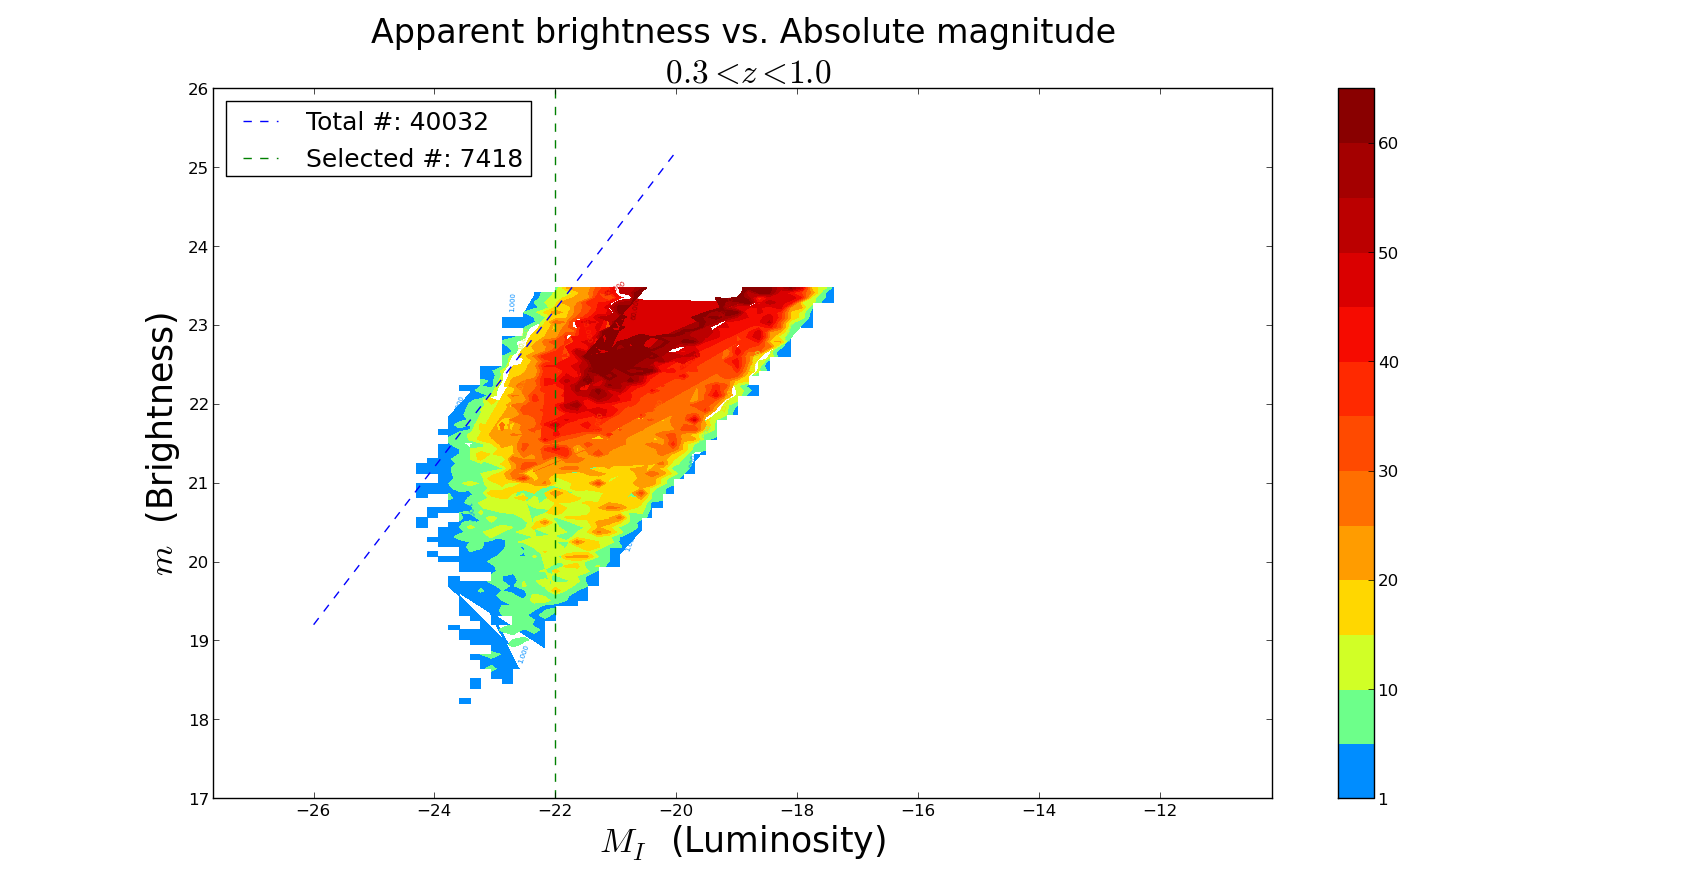
\includegraphics[width=\columnwidth]{fig1}
%   \label{fig:fig1}
%   \caption{}
% \end{figure}
% 
% {\bf Fig 2 - Histograms with diff MAG\_AUTO cuts}

\section{Methods}
\label{S:methods}
\subsection{Finding overdensities}
\label{sub:overdensities}
Every survey is flux-limited and so is COSMOS and is affected by Malmquist bias.
We generate, using the method below, a volume-limited sample that is complete upto $z=1$ by applying a cut on luminosity such that only galaxies instrinsically brighter than a certain threshold is considered.
Since the parent sample contains fainter galaxies, upto F814W=25.2, we compare the distribution of the F814W=23.5 sample with the samples containing fainter galaxies for high redshift bins, where the incompleteness affects first.
\begin{figure}
 \centering
 a) 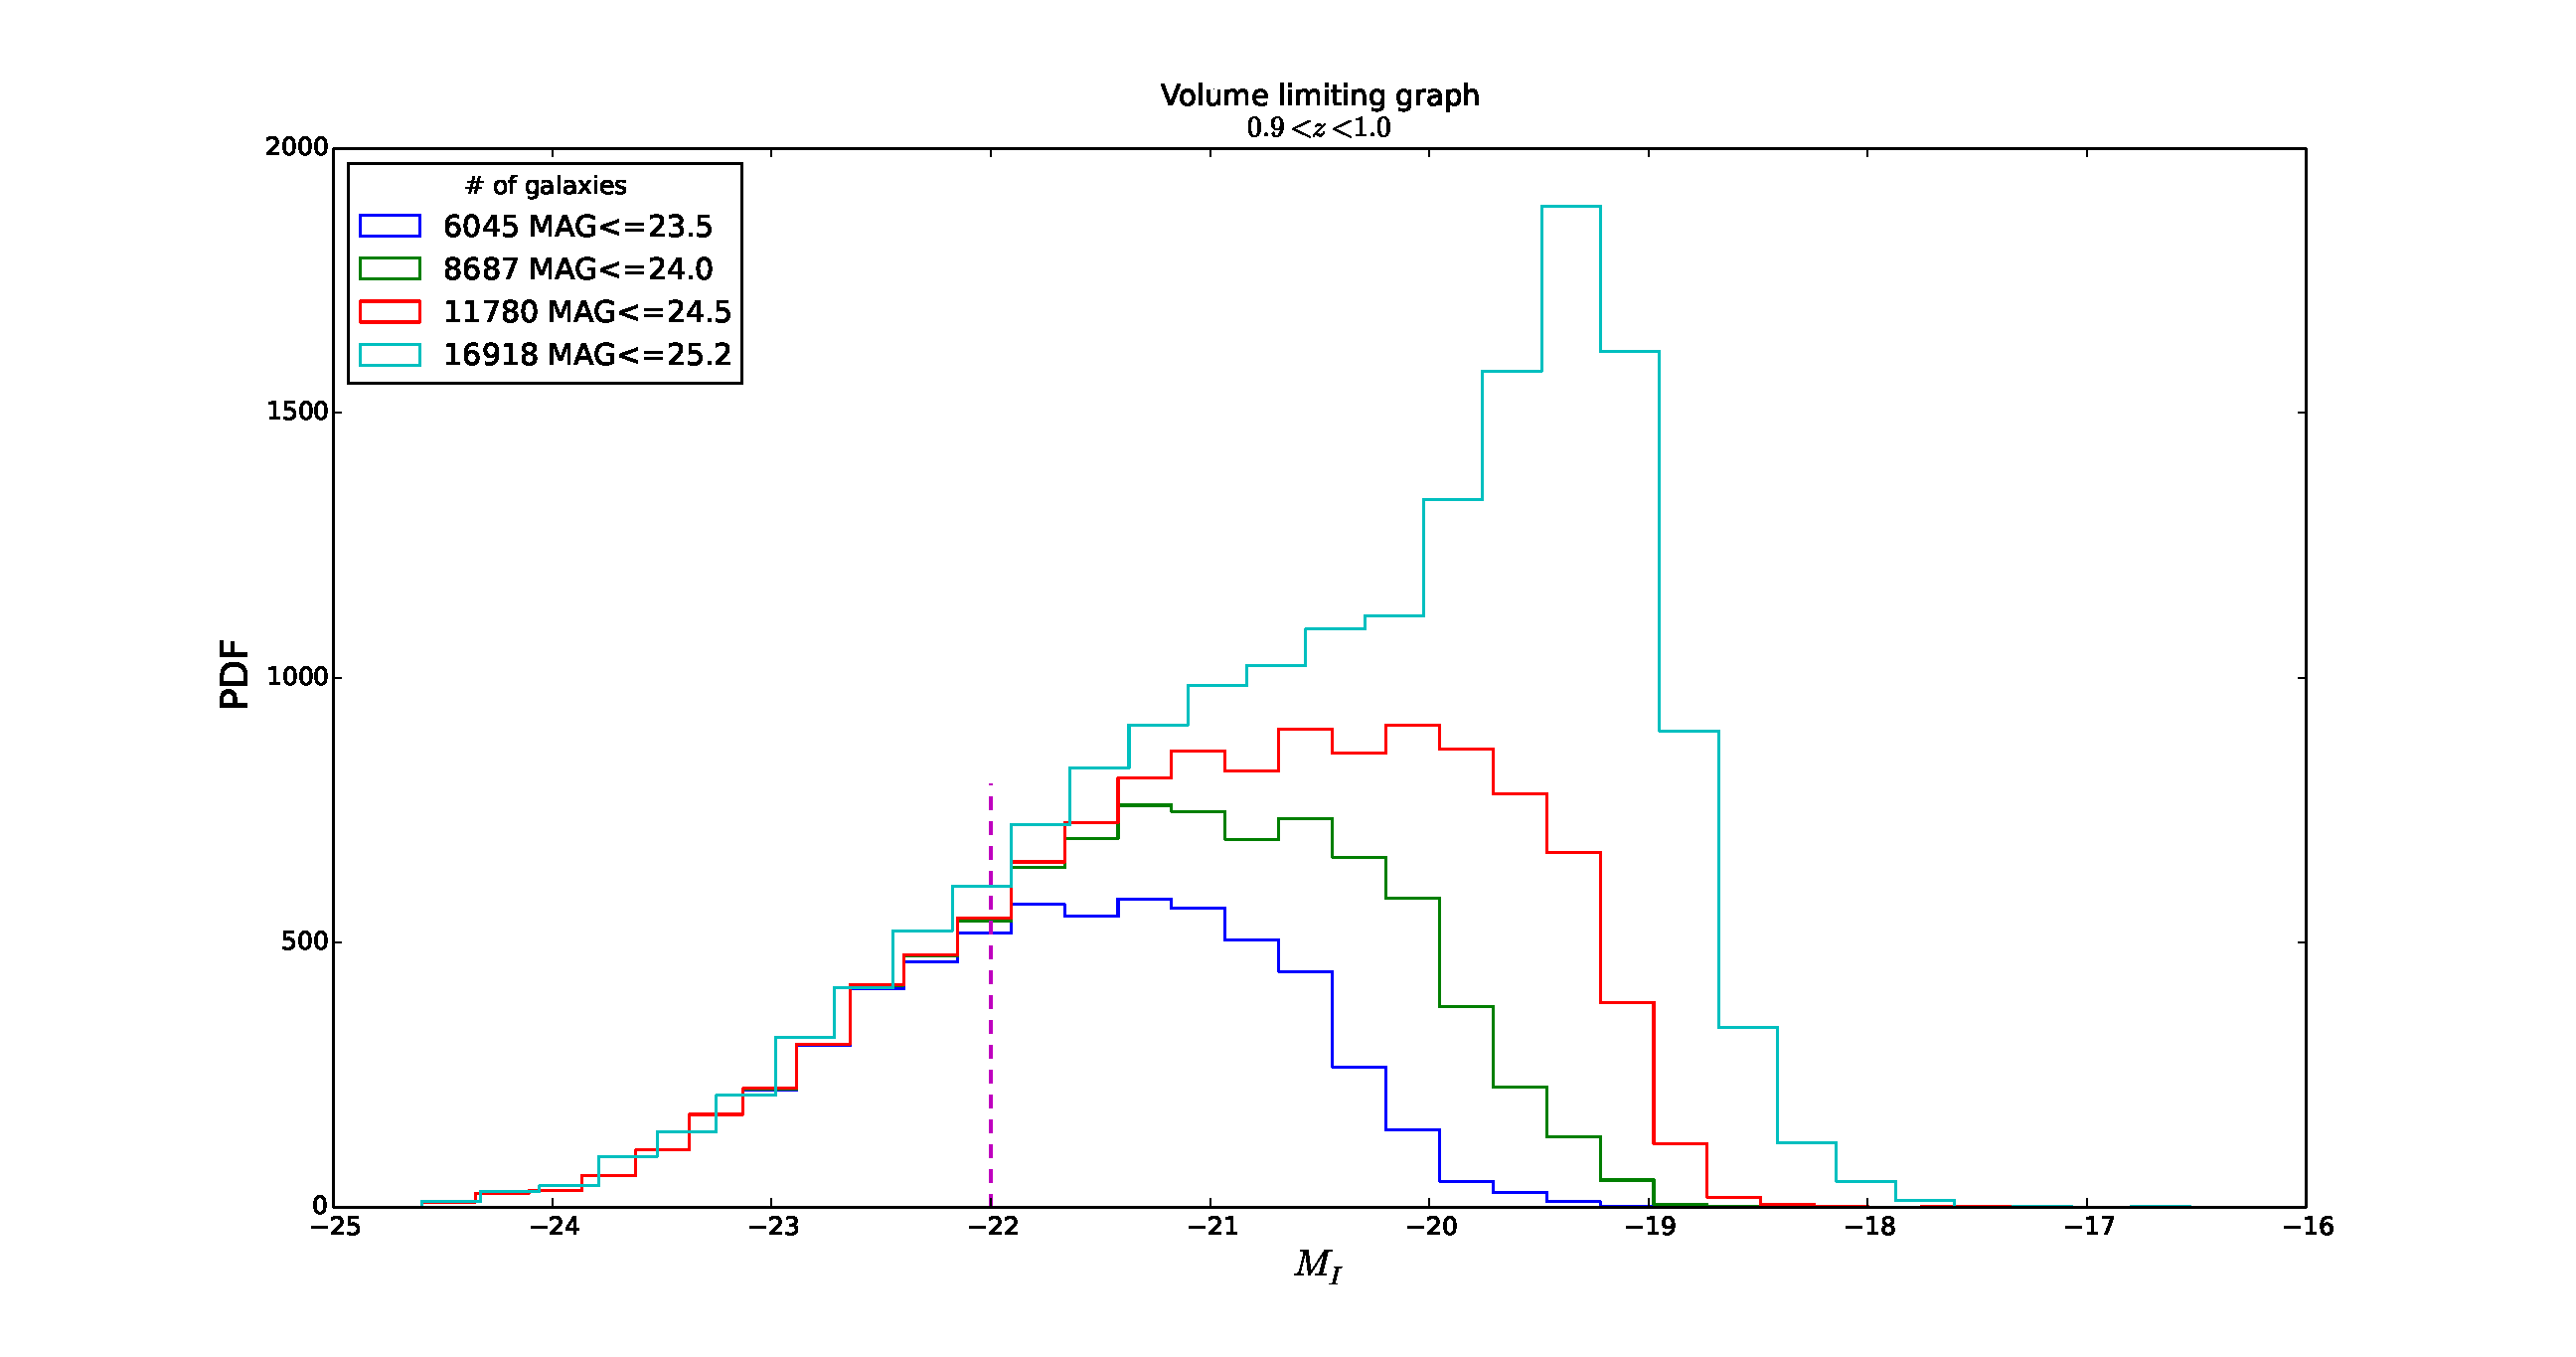
\includegraphics[width=\columnwidth]{volume_limiting_pdf}
 b) 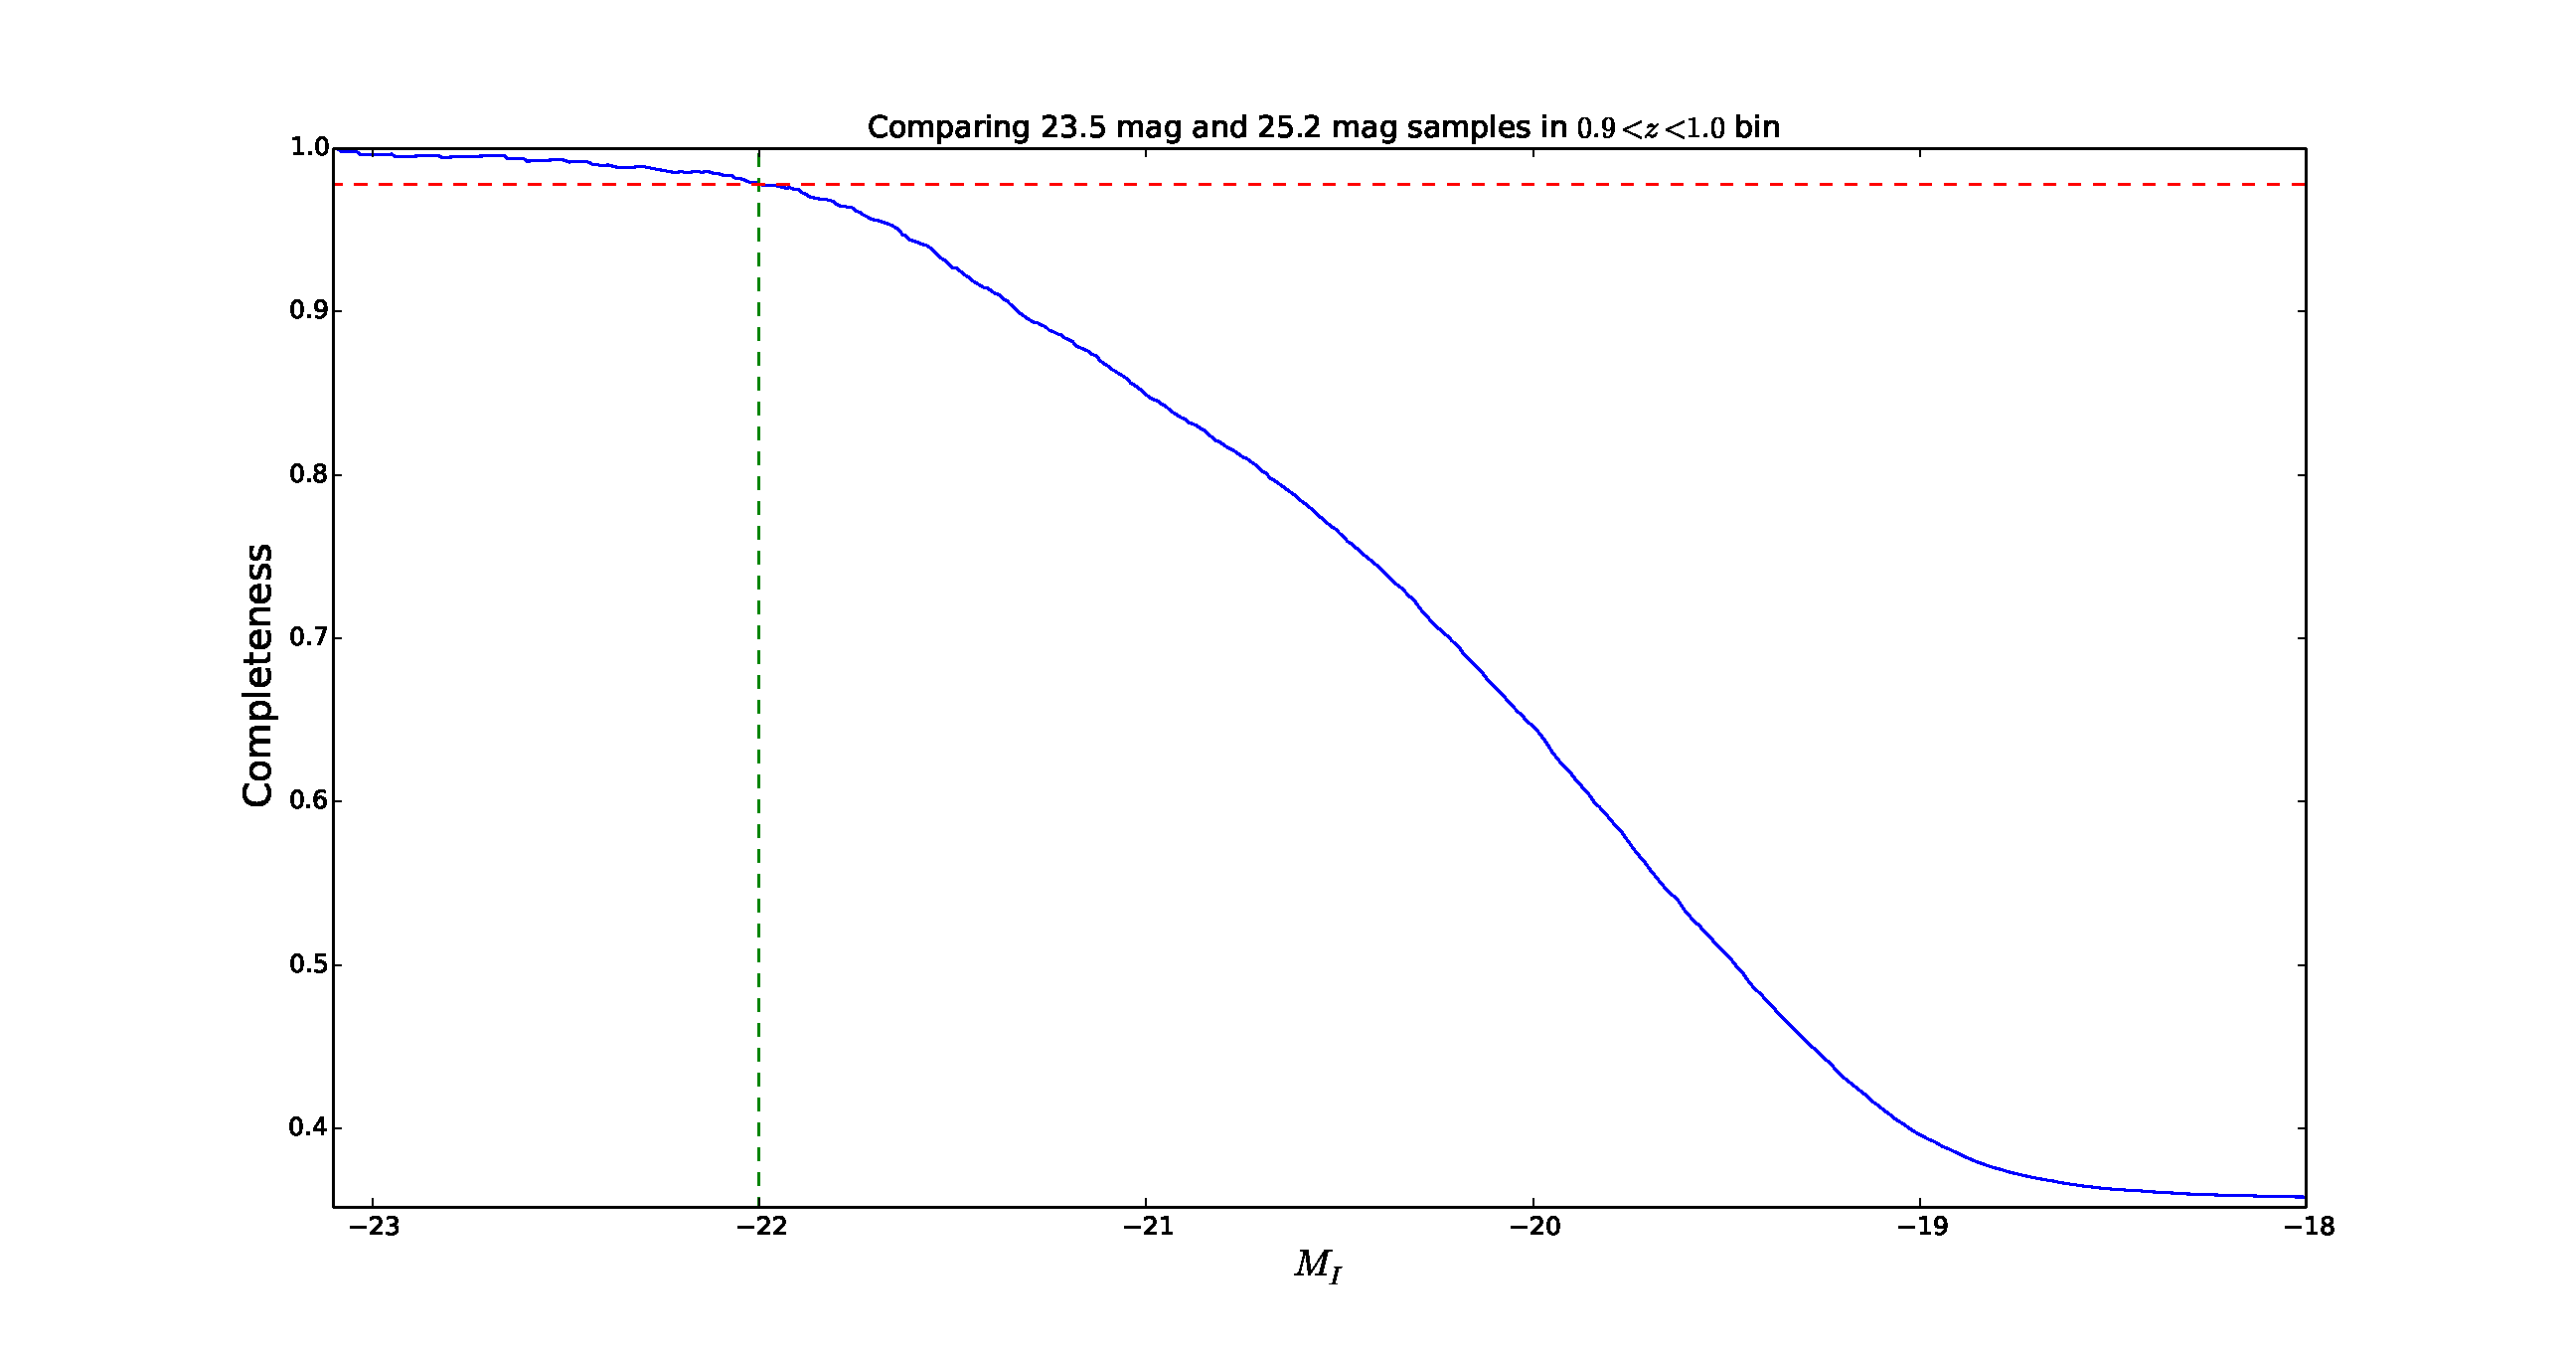
\includegraphics[width=\columnwidth]{volume_limiting_cdf}
 \label{fig:volume_limiting_dist}
 \caption{ ... }
\end{figure}

At $M_I\sim-22.0$, we see the sample is beginning to be biased in the $0.9<z<1.0$ bin due to the flux limit. We obtain 97.84\% completeness in this bin for $M_I$, where completeness is defined as the ratio between the number of galaxies in F814W$\le$23.5 and in F814W$\le$25.2 samples.
Fig.~\ref{fig:2Dhist} shows that at $M_I<-22$, we are not affected by flux limit yet. Note that not all galaxies in the sample have postage stamps.
Postage stamps may not exist either because the image occurs near the edge of the CCD chips or because the image is too large to fit in a bounding box. {\bf Rachel, please correct my terminology here.}
While the former is purely random and doesn't introduce bias, the latter is not. Typically galaxies that are nearby and intrinsically very bright do not have postage stamps associated with them. However,
However, since we used the F814W$\le$23.5 sample, irrespective of the existence of postage stamps, we believe that our conclusions are not affected by this bias.

\begin{figure}
  \centering
   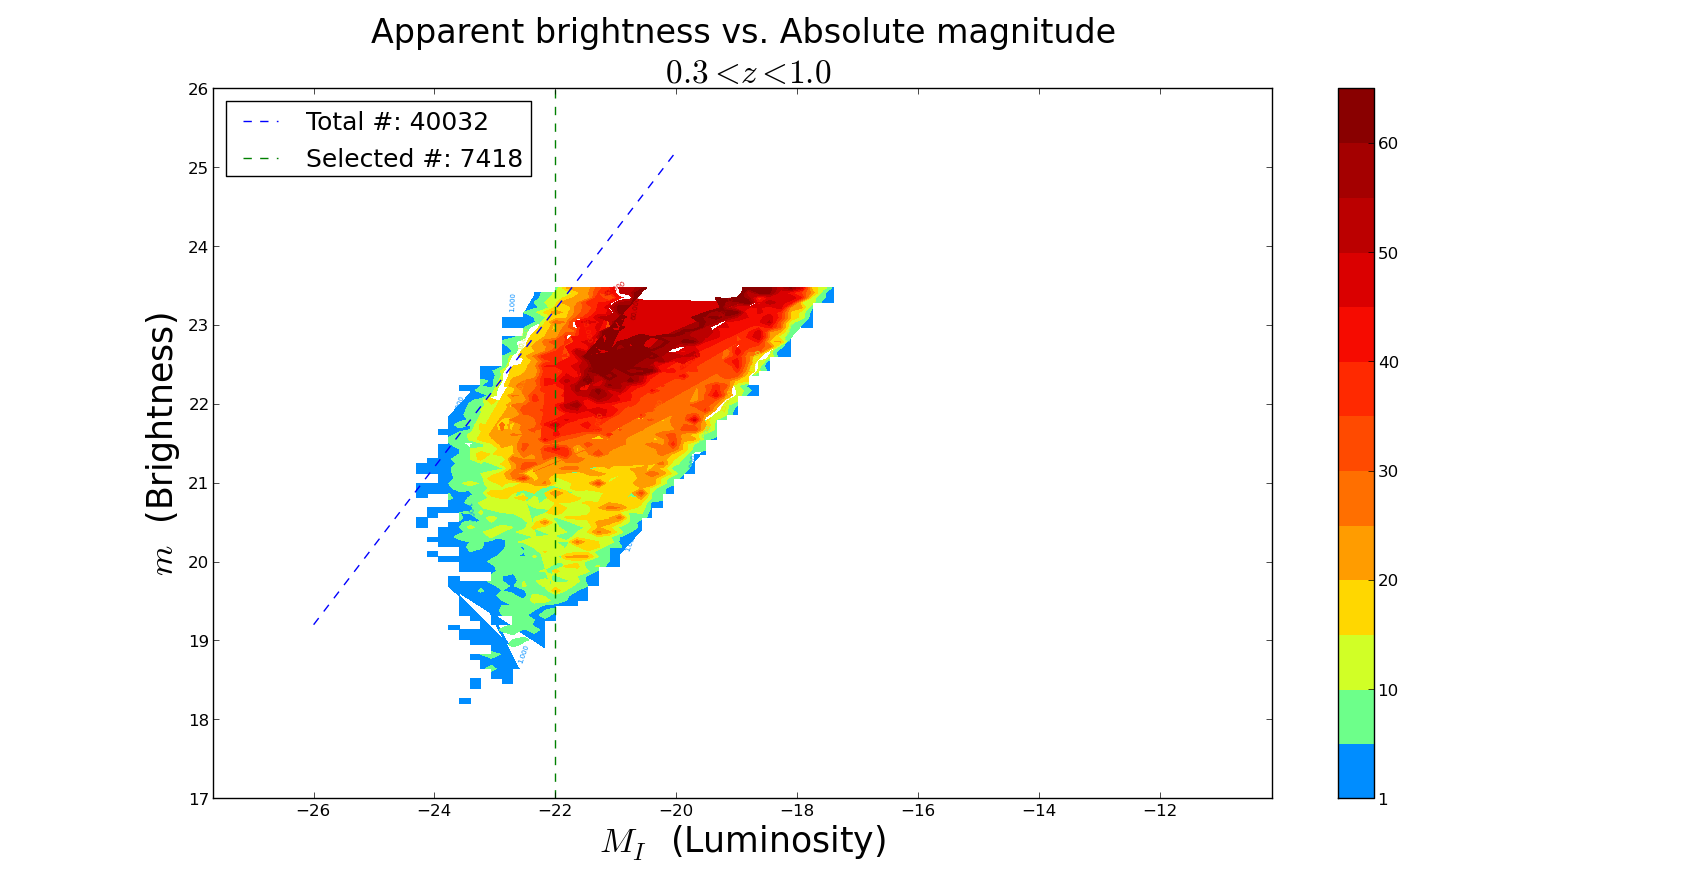
\includegraphics[width=\columnwidth]{fig1}
   \caption{2-D histogram of galaxies in apparent magnitude ($m$) and absolute magnitude ($M_I$) space.}
   \label{fig:2Dhist}
 \end{figure}

 
In a wide-field survey, regions of overdensities are identified by computing 3-dimensional comoving densities. But in narrow field surveys like COSMOS, previous work {\bf cite } have shown
that regions of overdensities can be identified from a 1-dimensional histogram of redshifts, at least for low redshifts. 

For our sample of galaxies, volume-limited upto $z=1$ by imposing an $M_I$ cut, we fit parametric models to the histogram of photometric redshifts in order to assign values of overdensity. The figures show chi-squared and gamma functions fitted to the histogram~\citep{Redshift_modelling}.
For low $z$, the volume is too small to rely the overdensity values from our model fits and hence the fit is made for $z>=0.3$. Our binning width, $\Delta z$ must be small enough so as to be able to identify localized overdensities/underdensities but large enough to not let our conclusions be affected by the errors in photometric redshift. 
We choose our bins to be $0.05$ wide starting from $z=0.3$. 

The curves are normalized such that the area under the curves is equal to the number of galaxies considered.
{\bf Fig 3 - Histogram with fits }. \\
\begin{figure}
 \centering
  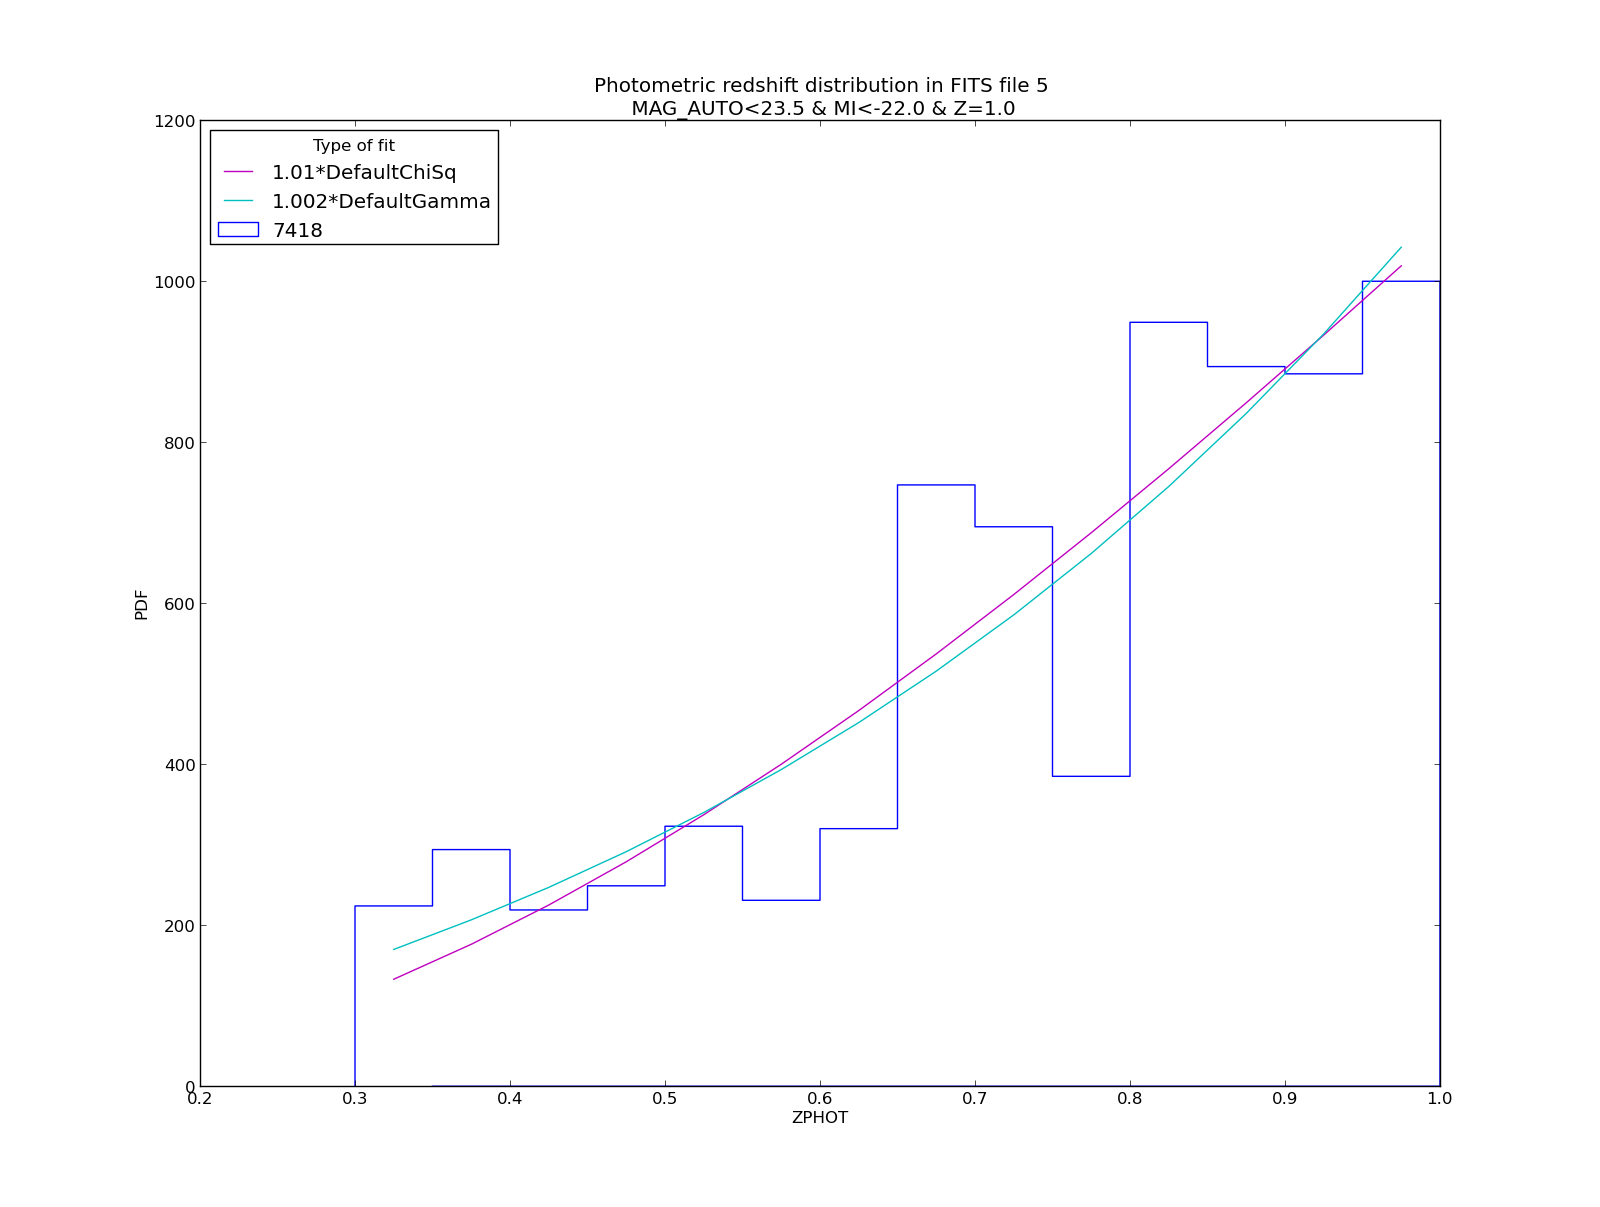
\includegraphics[width=\columnwidth]{fig3}
  \label{fig:fig3}
  \caption{}
\end{figure}

Overdensity in a redshift bin is defined as the ratio of the difference between the value given by the histogram and the value predicted by the model to the latter: $\delta=(N-N_{\text{mod}})/N_{\text{mod}}$. 
We leave a 10\% margin of safety i.e. ff $\delta$ from both the fits is greater than $0.1$, then we call that redshift bin as an
overdense region whereas if $\delta$ from both the fits is less than $-0.1$, then we call that as an underdense region. Redshift bins with $-0.1 < \delta < 0.1$ are neither too overdense
nor too underdense and we call them as `unclassified regions'  and discard them from our analysis.{\bf Fig 4 - overdensities vs redshift bins}.

\begin{figure}
 \centering
 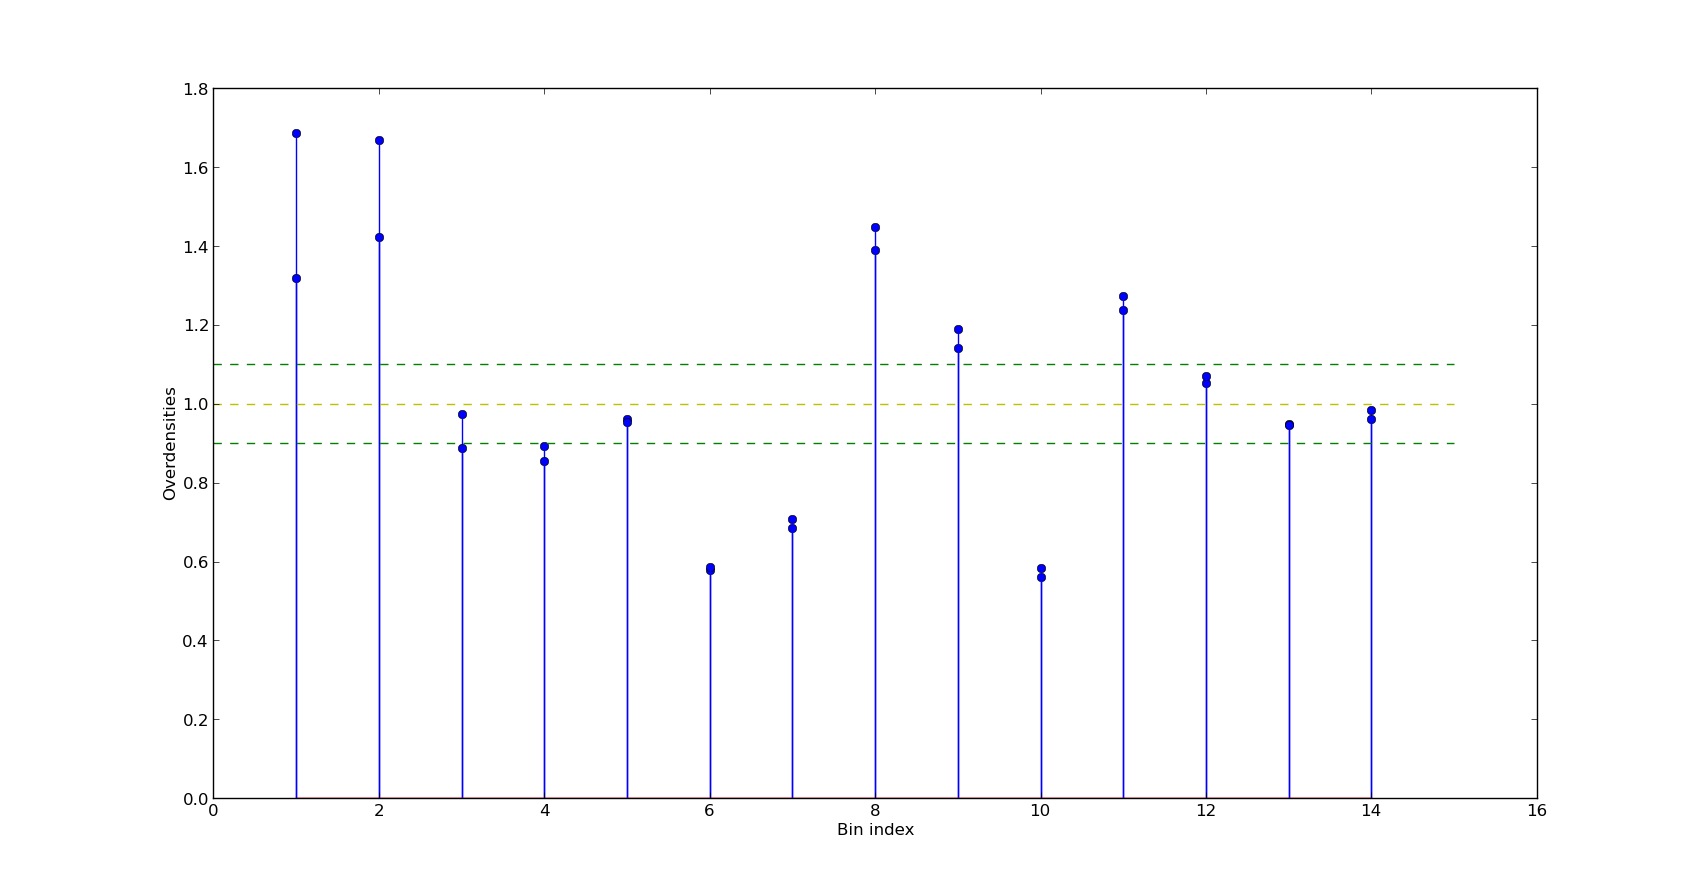
\includegraphics[width=\columnwidth]{fig4}
 \label{fig:fig4}
 \caption{}
\end{figure}

While this may seem arbitrary, the overdense and underdense regions obtained by the above method have local average number density higher than the global average number density. Refer to Figure~\ref{fig3}.
We thus identify the regions $z=0.30-0.40, 0.65-0.75, 0.80-0.85$ as overdense, $z=0.55-0.65, 0.75-0.80$ as underdense and $z=0.40-0.55$ as unclassified.
The classification of overdensities and underdensities agrees with the work done by~\cite{Kovac_Density10k} except for the last two redshift bins. 

We see that the region between $0.85<z<1.0$ is neither overdense nor underdense according to our model and hence is not going to be considered for further analysis.

We use therefore relax our luminosity cut %to $-20.8$
so that the sample is volume-limited \emph{not} until $z=1$ but until $z=0.85$. This increases the sample size significantly.
We choose to impose the cut at $M_I=-20.8$, with 95\% completeness. 

Refitting the model to our new sample is consistent with the previous assignment of overdensities.


\begin{tabular}{c|c|c|}
 \hline
 Redshift & \# of galaxies & Environment \\
 \hline
 0.30-0.35 & 726 & Overdense \\
 0.35-0.40 & 1000 & Overdense \\
 0.55-0.60 & 727 & Underdense \\
 0.60-0.65 & 1070 & Underdense \\
 0.65-0.70 & 2089 & Overdense \\
 0.70-0.75 & 1970 & Overdense \\
 0.75-0.80 & 1159 & Underdense \\
 0.80-0.85 & 2428 & Overdense \\
 \hline
\end{tabular}

\begin{figure}
 \centering
 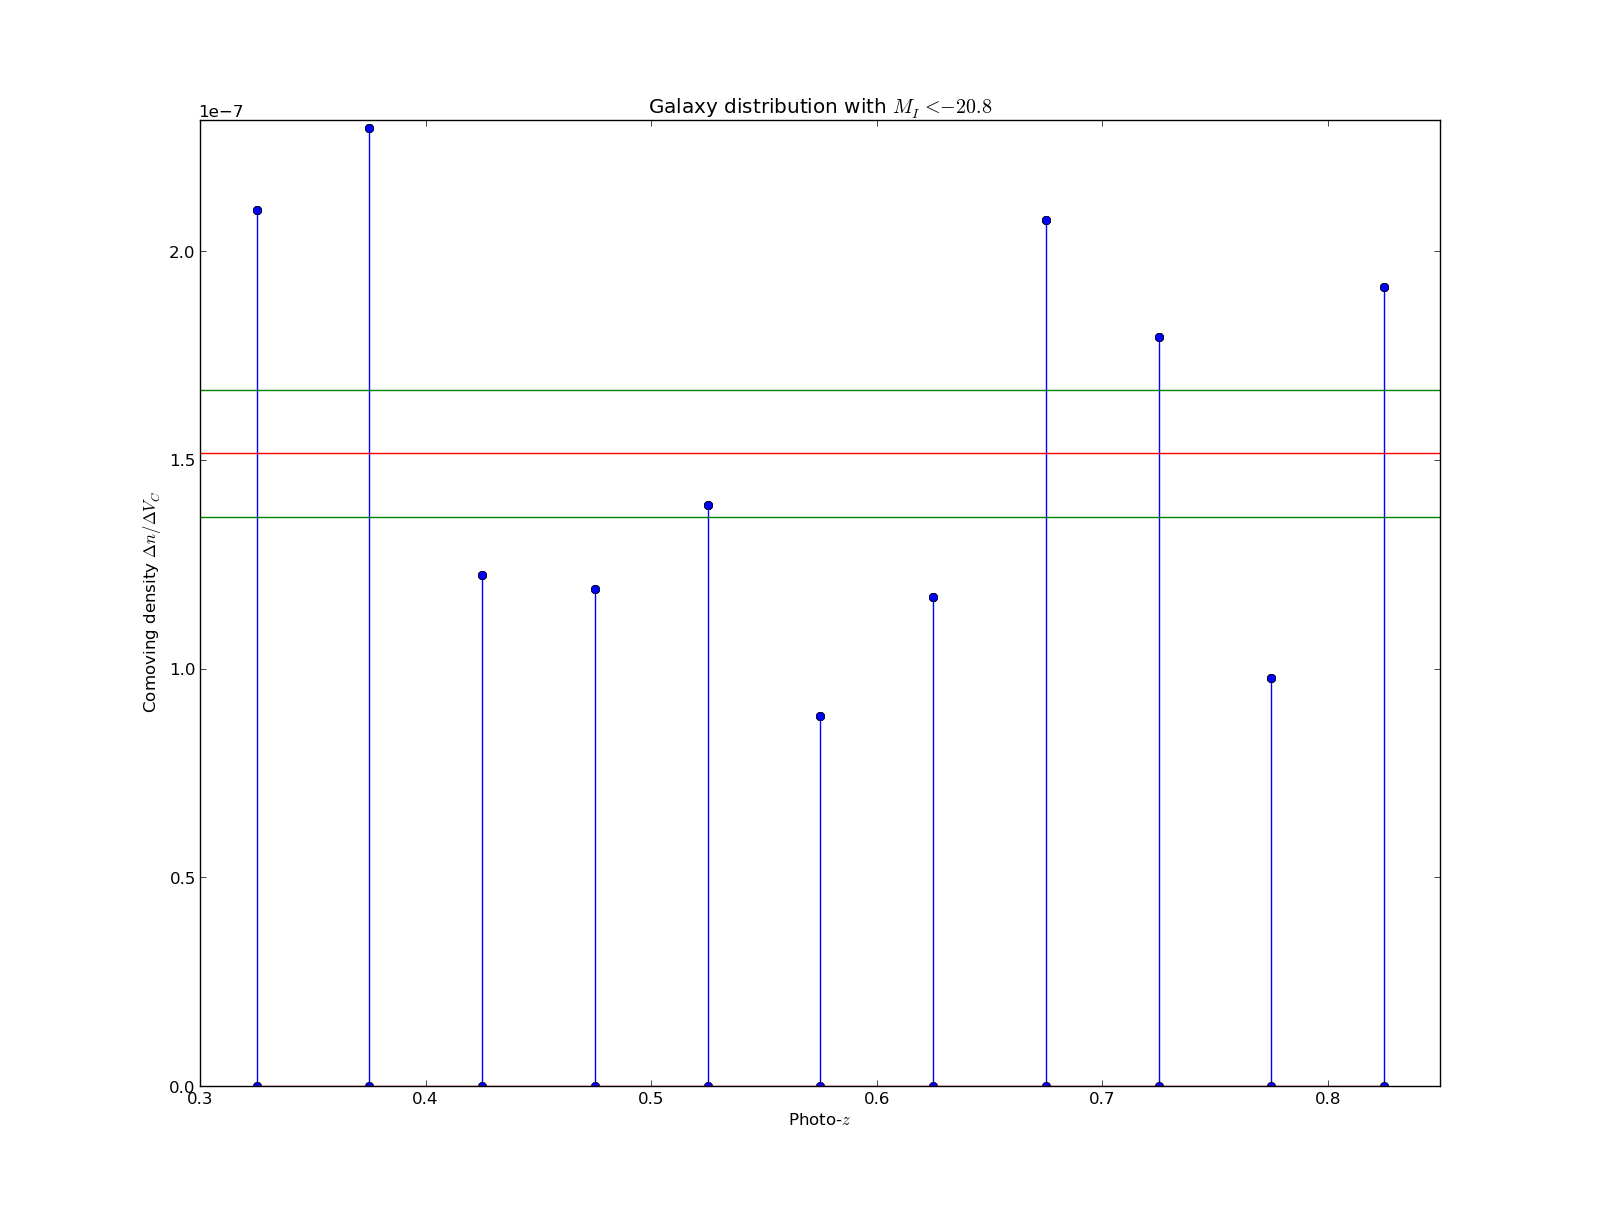
\includegraphics[width=\columnwidth]{../plots_20140219/comoving_densities(2b).png}
 \label{fig:comoving_densities}
 \caption{}
\end{figure}

In the following section, we will compare and analyze the distribution of properties of the galaxies residing in the overdense regions.

%
%\subsection{Correcting for SNR} 
%{\bf Fig 5 - hist\_magauto }. As seen in Fig 5, the overdense and the underdense regions differ in their brightness distributions. This translates to the overdense and the underdense regions 
%having different Signal-to-Noise ratios (SNR) and we need to correct for it. The fits are better for brighter galaxies and not as good for fainter ones. And there is a higher
%fraction of fainter galaxies in the underdense regions than in the overdense regions. To avoid any bias creeping in due to this, weights are assigned
%to the galaxies in the underdense regions such that
%the distributions of the brightness (MAG\_AUTO) scale to become identical. All other histograms that follow in this section are weighted.

\emph{Talk more about environments - Nature and nurture?}

%\section{Implications/Comparisons}
%\section{Results}
\subsection{Finding axis ratios $(b/a)$}
\label{s:axisratio}
{\bf Should explain in brief Claire's work.} \\
If galaxies have elliptical isophotes, its shape and size could be defined by the axis ratio and the area enclosed by a boundary isophote. However, in real galaxy images,
the boundary may not be well defined and the shape may not be well approximated by an ellipse. Given the surface brightness (intensity) $I(\vec{\theta})$ of a galaxy image at every angular position $\vec{\theta}$,
we can define the tensor of second brightness moments as
\begin{equation}
 Q_{ij} = \frac{\int\rmd^2\theta q_I (\theta_i - \overline{\theta_i})(\theta_j - \overline{\theta_j})}{\int\rmd^2\theta q_I},
\end{equation}
where $q_I$ is a suitable chosen kernel and $\overline{\vec{\theta}}$ is the average angular coordinate, weighted by the same kernel function and $i,j\in\lbrace 1,2 \rbrace$ are the componenets of $\vec{\theta}$.
It is common to find in literature two kinds of \emph{complex }ellipticities that quantify the shape of the galaxies - $\chi$ and $\epsilon$ defined as
\begin{align}
 \chi &= \frac{Q_{11}-Q_{12}+2iQ_{12}}{Q_{11}+Q_{22}} \\ \epsilon &= \frac{Q_{11}-Q_{22}+2iQ_{12}}{Q_{11}+Q_{22}+2(Q_{11}Q_{22}-Q_{12})^{1/2}}
\end{align}
If the image has elliptical isophotes with axis ratio $q$, then 
\begin{align}
 |\chi| &= \frac{1-q^2}{1+q^2}, \\ |\epsilon| &= \frac{1-q}{1+q}. 
\end{align}

Conversely, if we can compute $\chi$ or $\epsilon$ for a galaxy, we can obtain an effective, azimuthally averaged {\bf(?)} axis-ratio $q$. 
The distribution of the axis ratios that are obtained by the above manner are compared between redshift bins. We use two statistical tests namely the Kolmogorov-Smirnov test and Anderson-Darling test to compare distributions.
\begin{figure}
 \centering
 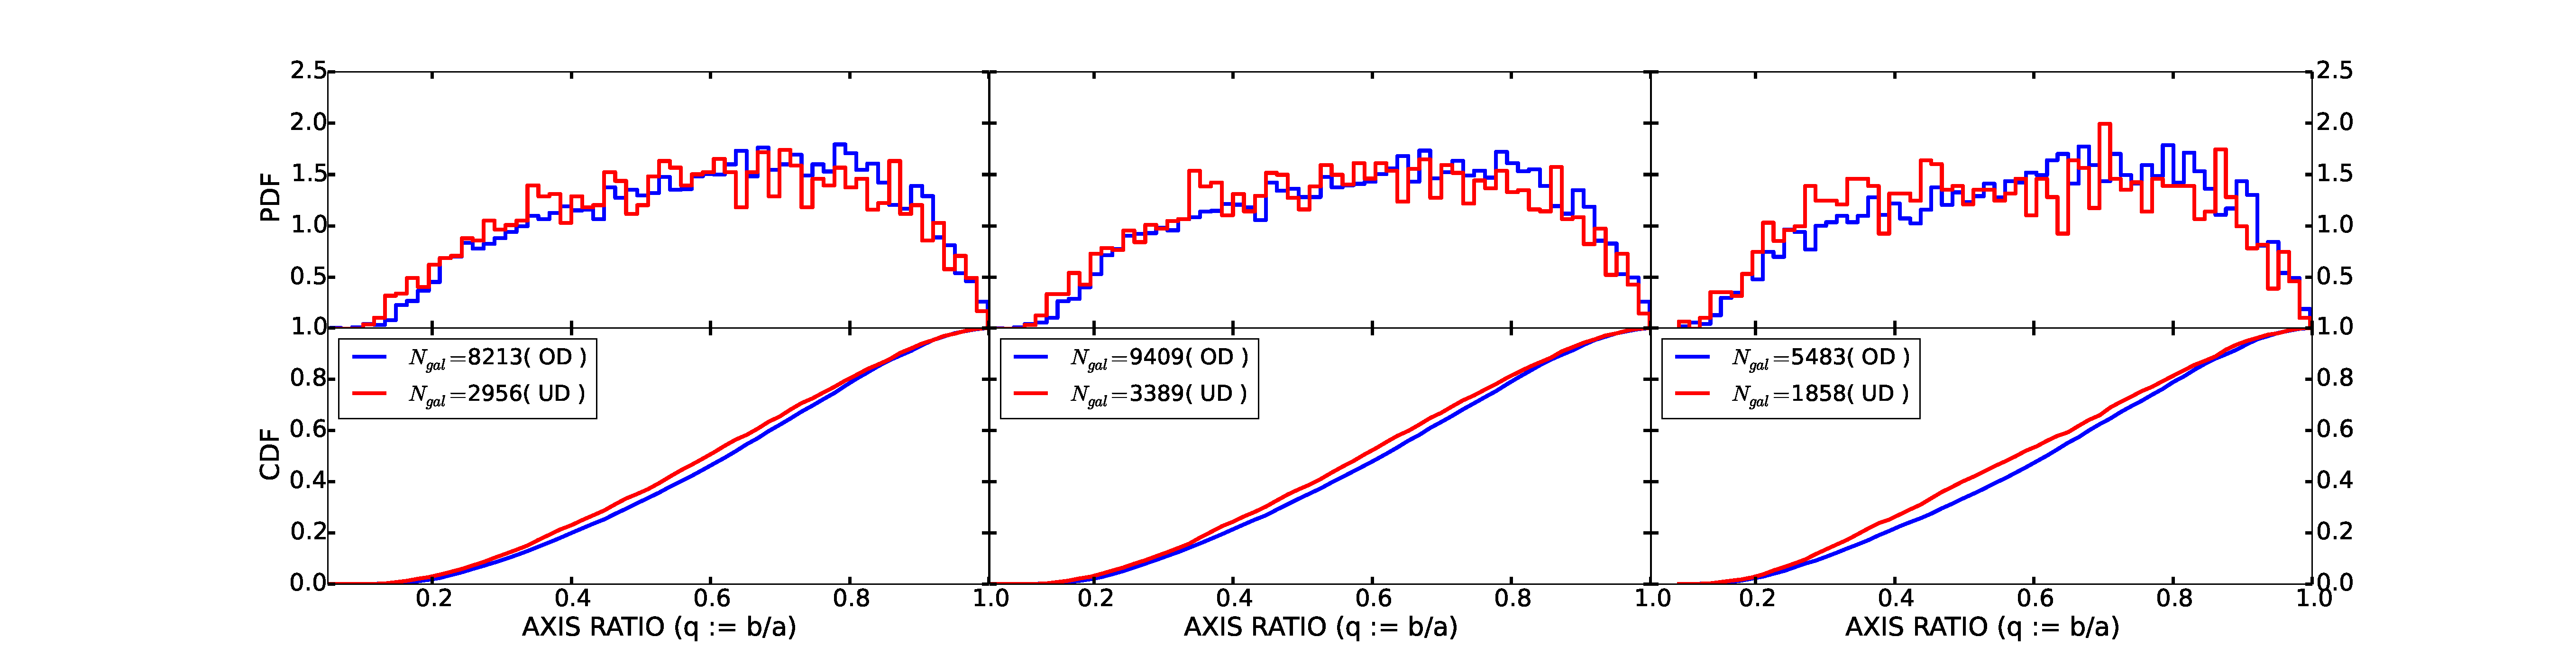
\includegraphics[width=\columnwidth]{axis_ratio_all.eps}
 \caption{KS p-value = 0.004 \& AD p-value = 0.001}
 \label{fig:axisratio_all}
\end{figure}

We first compare the distribution of the axis ratio in \emph{all} overdense bins and \emph{all} underdense bins. The p-value from both the KS and AD tests are below 0.05, 
so we believe (95\% level) in the `alternate hypothesis' that the overdense and underdense regions have different axis ratio distributions.
Figures~\ref{fig:axisratio_similar} and~\ref{fig:axisratio_contrasting} do a similar comparison bin-wise and show that the distributions are similar when the environments are similar and different when the environments are different.
The cumulative distinction functions are also plotted alongside in order to be able to visualize the `distance' between the distributions.


\begin{figure*}
 \centering
 a) 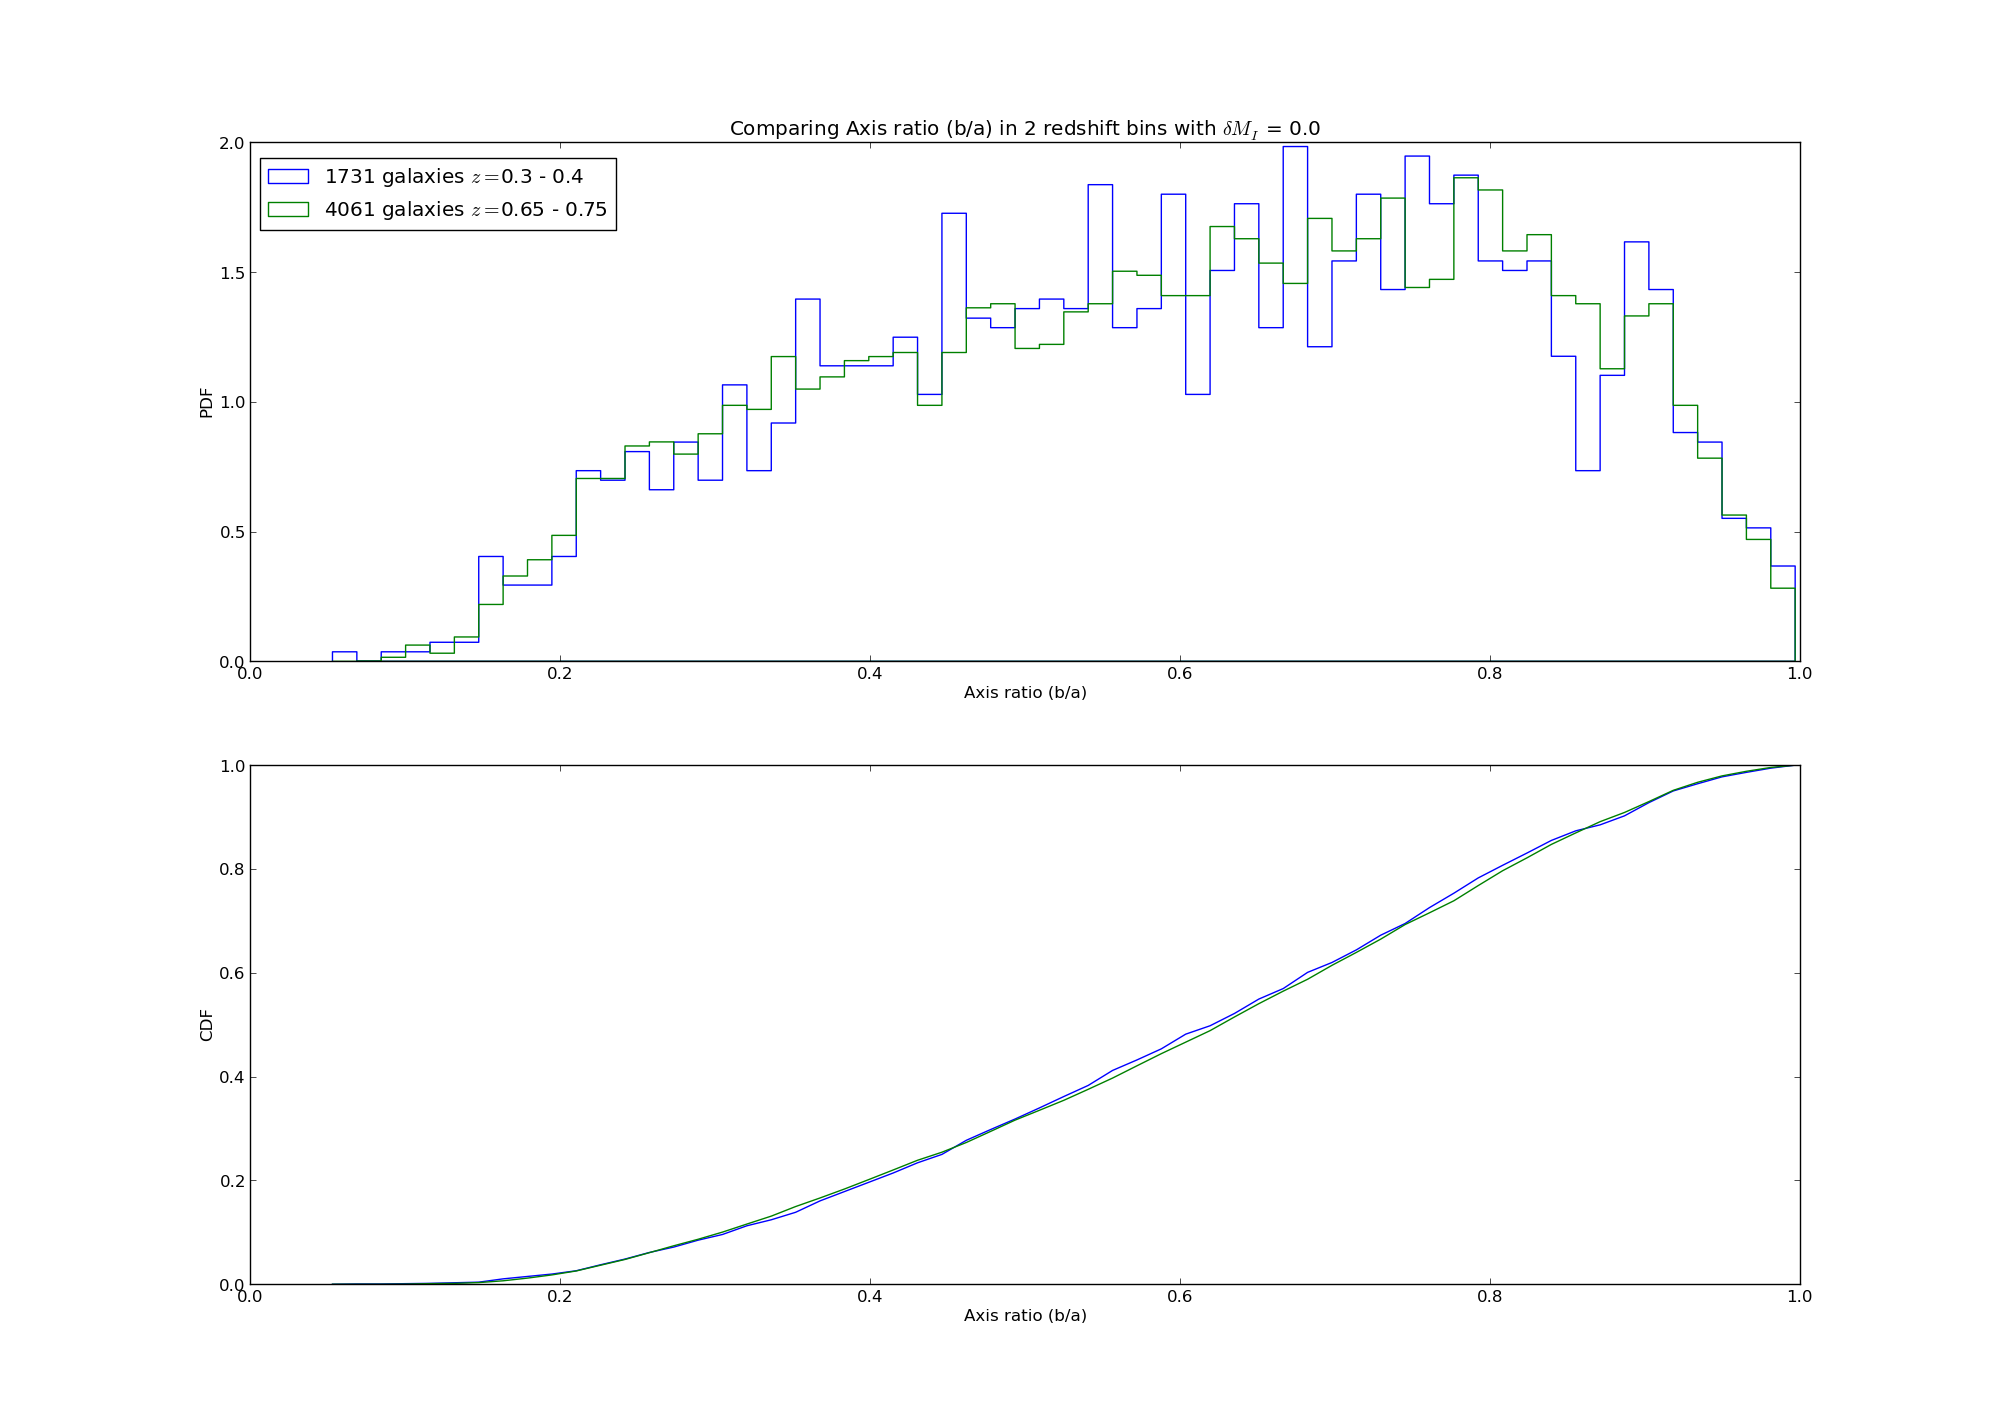
\includegraphics[width=0.9\columnwidth]{axisratio(0)_0dot3-0dot4_0dot65-0dot75.png} \
 b) 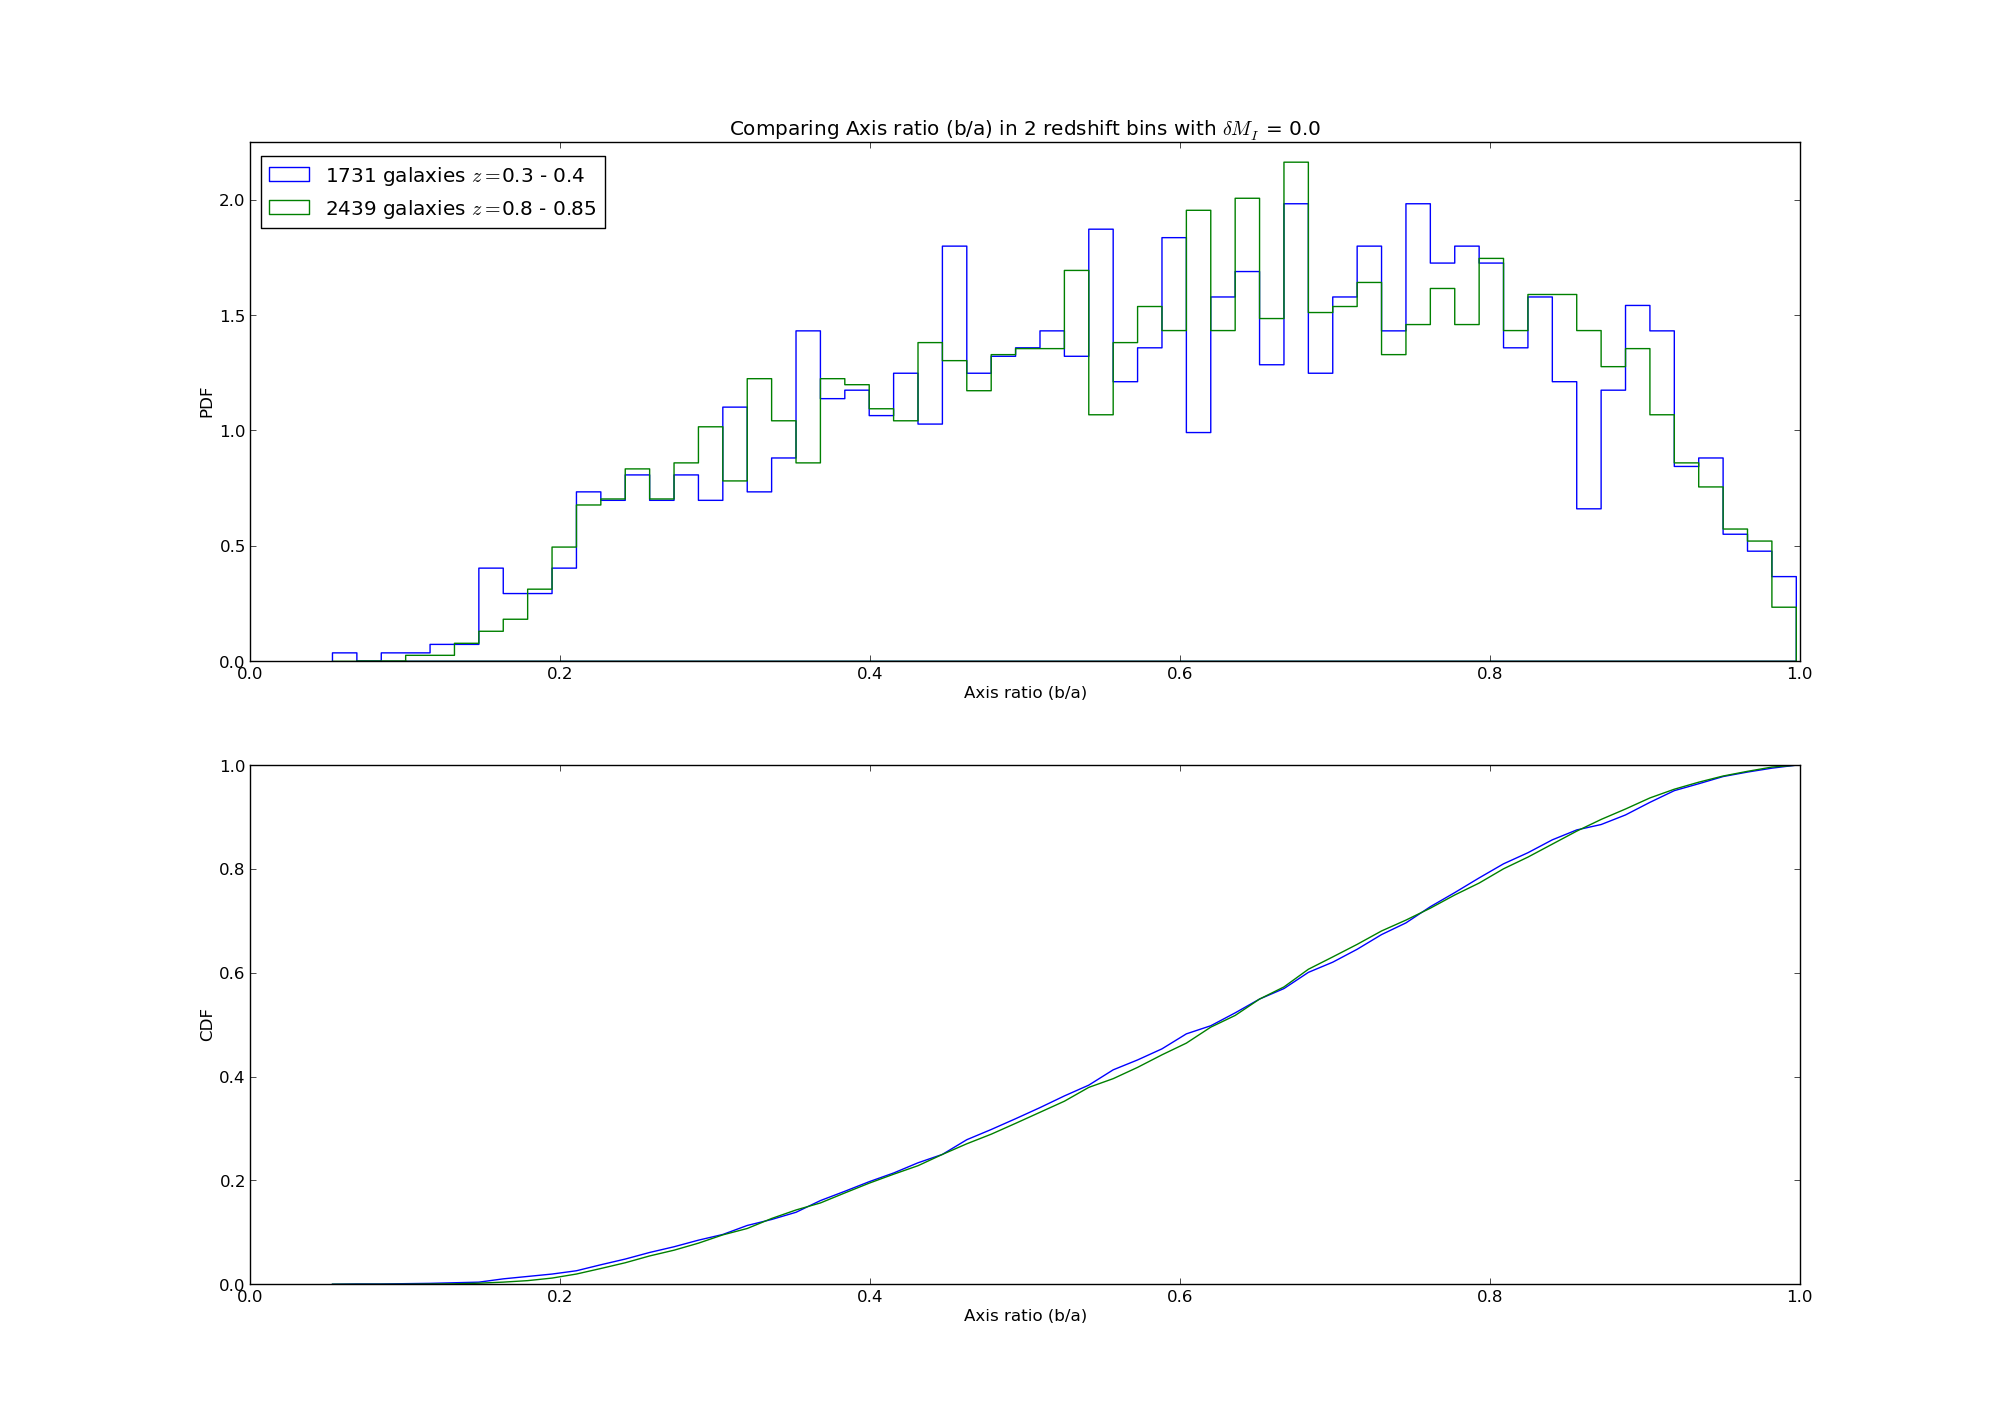
\includegraphics[width=0.9\columnwidth]{axisratio(0)_0dot3-0dot4_0dot80-0dot85.png} \\
 c) 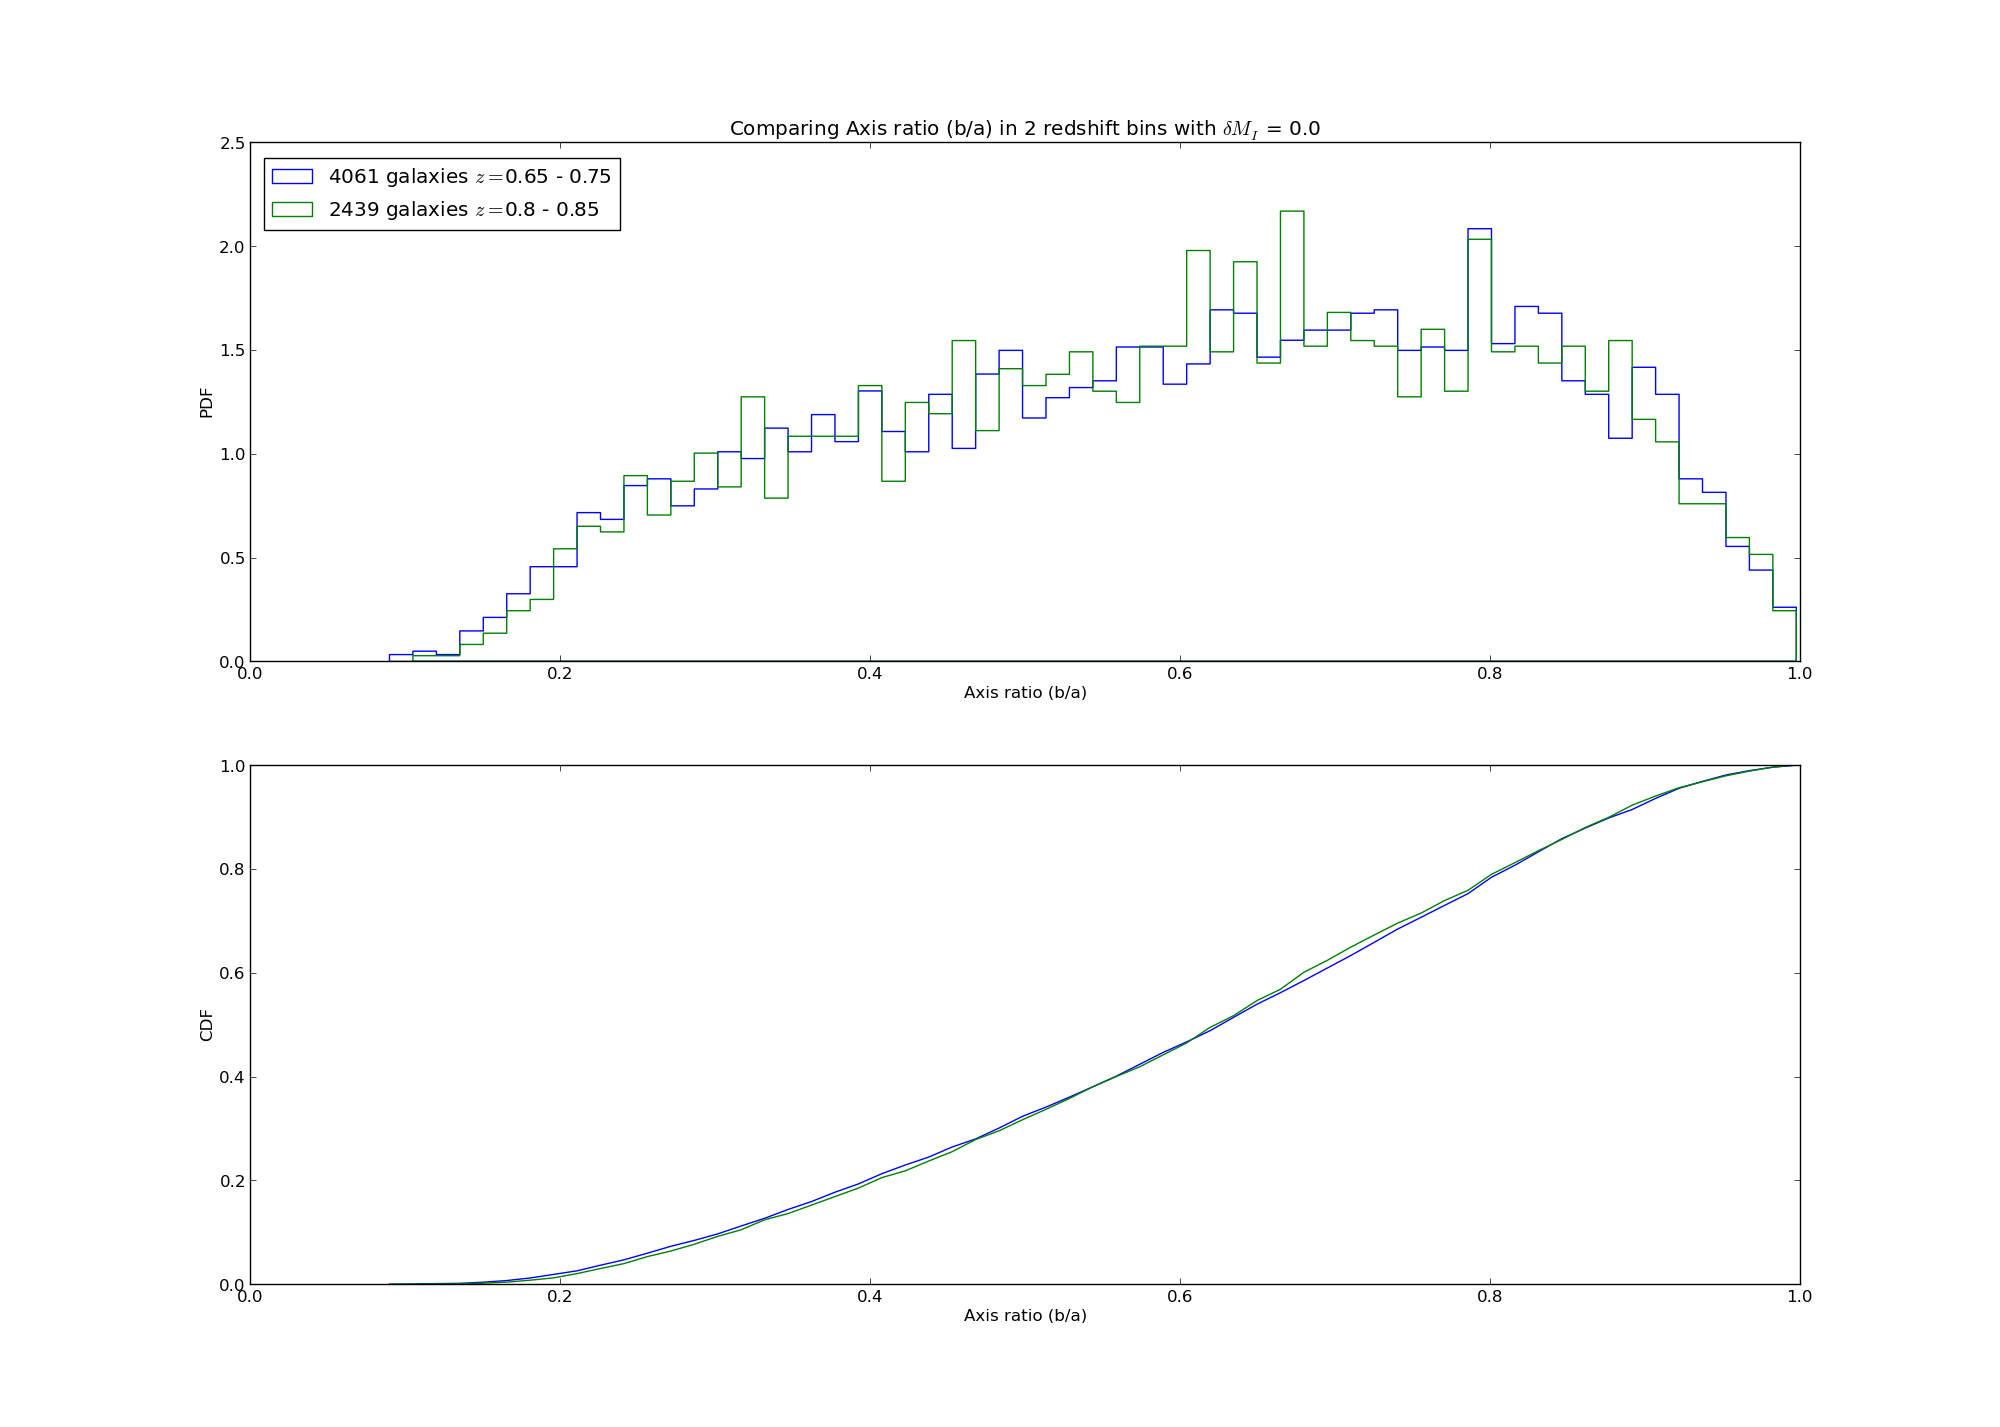
\includegraphics[width=0.9\columnwidth]{axisratio(0)_0dot65-0dot75_0dot8-0dot85.png} \
 d) 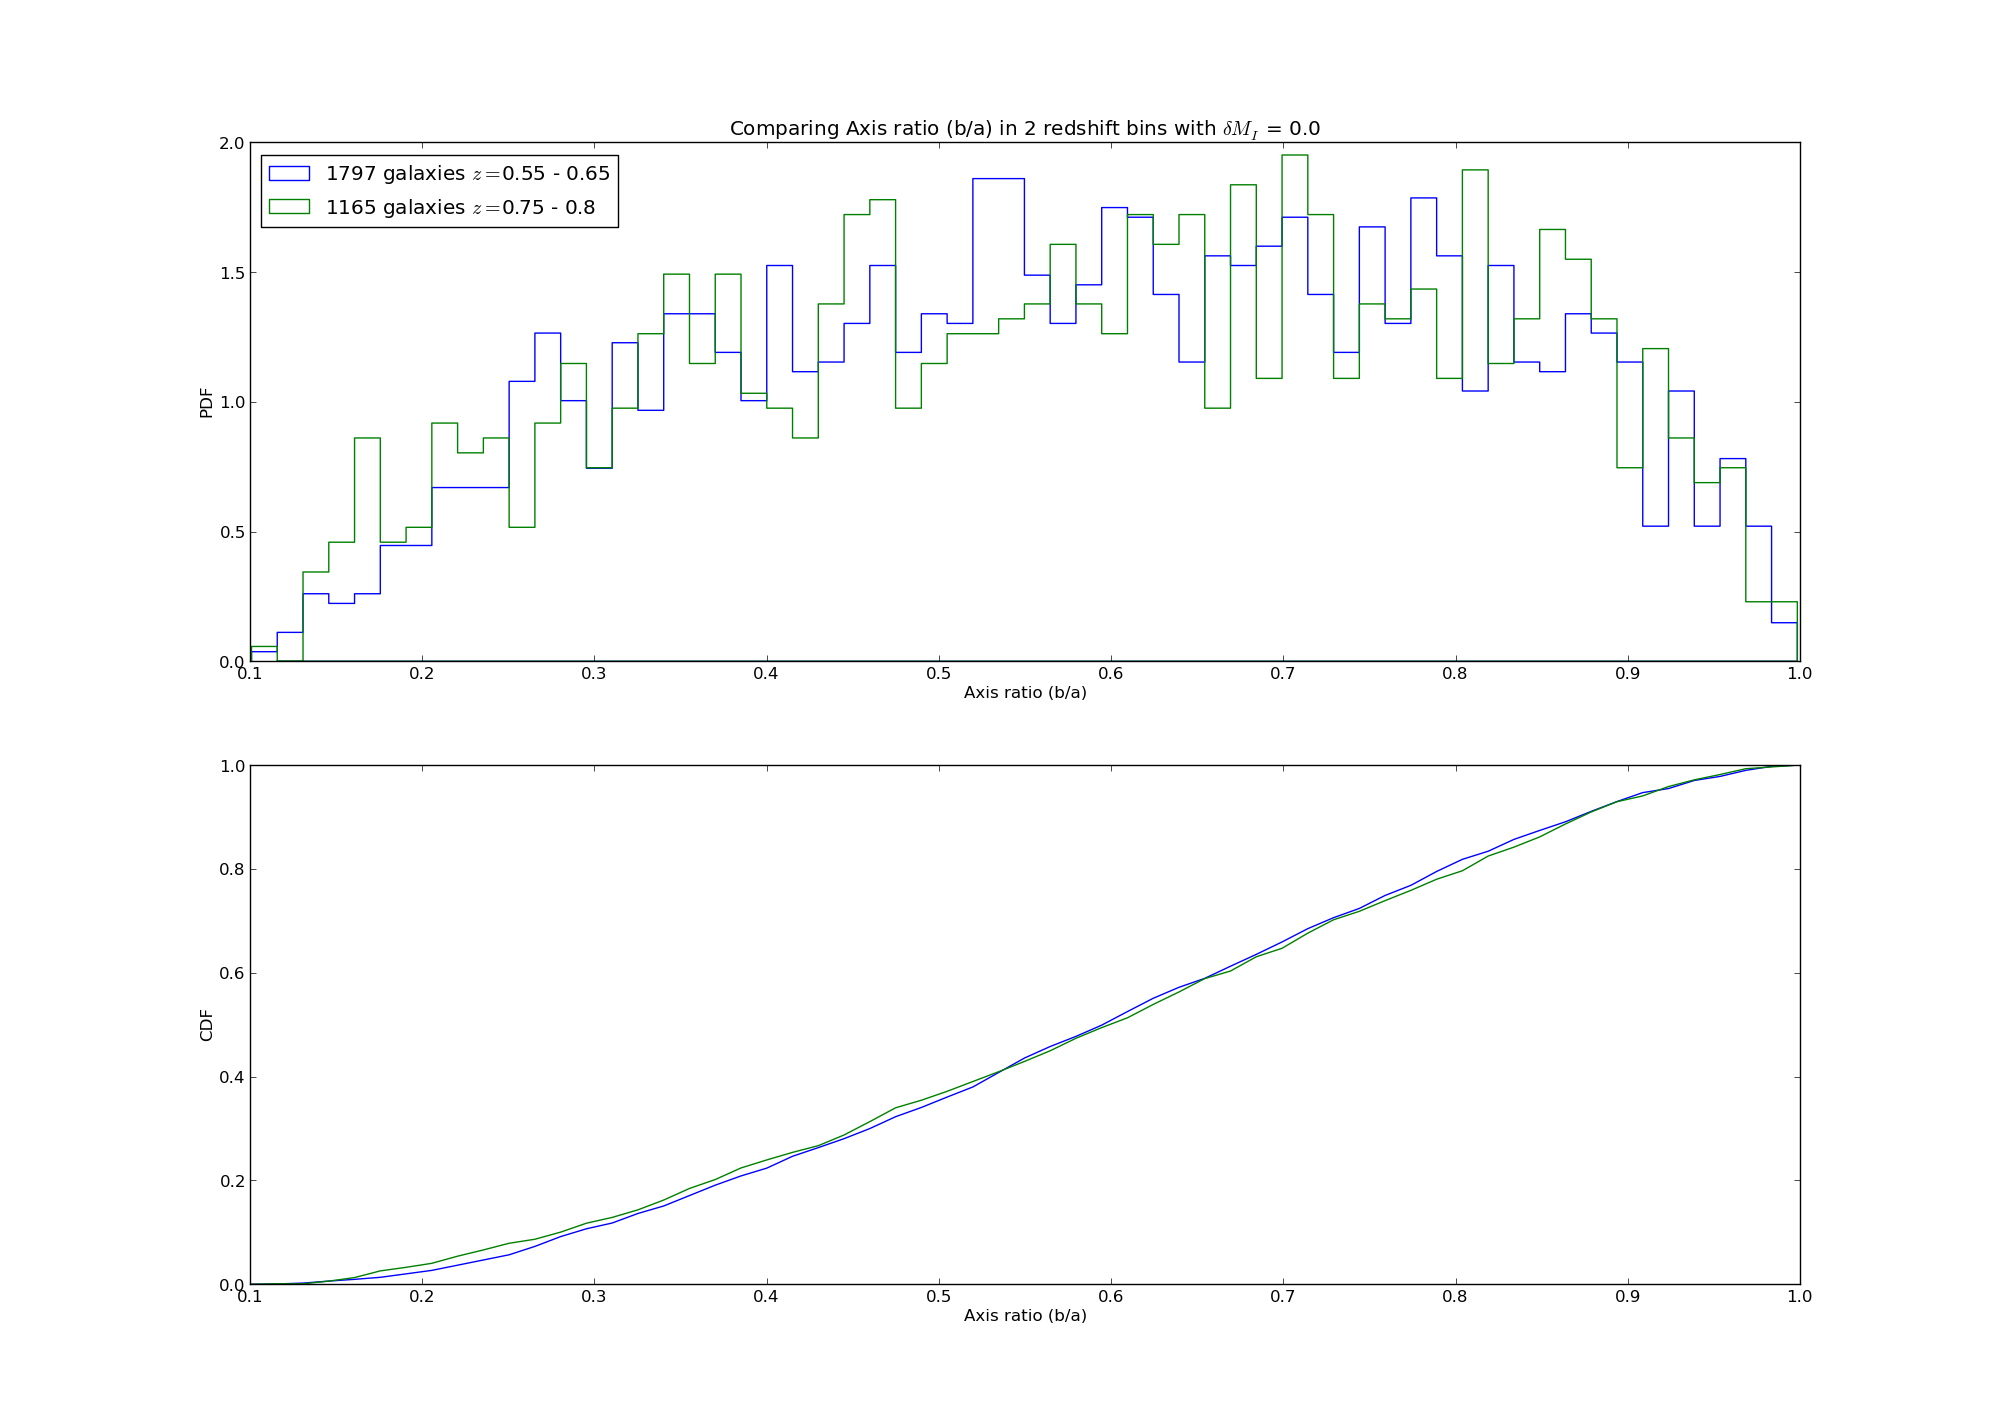
\includegraphics[width=0.9\columnwidth]{axisratio(0)_0dot55-0dot65_0dot75-0dot8.png} \
 \caption{Comparison of axis ratios of galaxies in similar environments. $p$-values from the KS and AD test are (will be) given in the plot.}
 \label{fig:axisratio_similar}
\end{figure*}

\begin{figure*}
 \centering
 a) 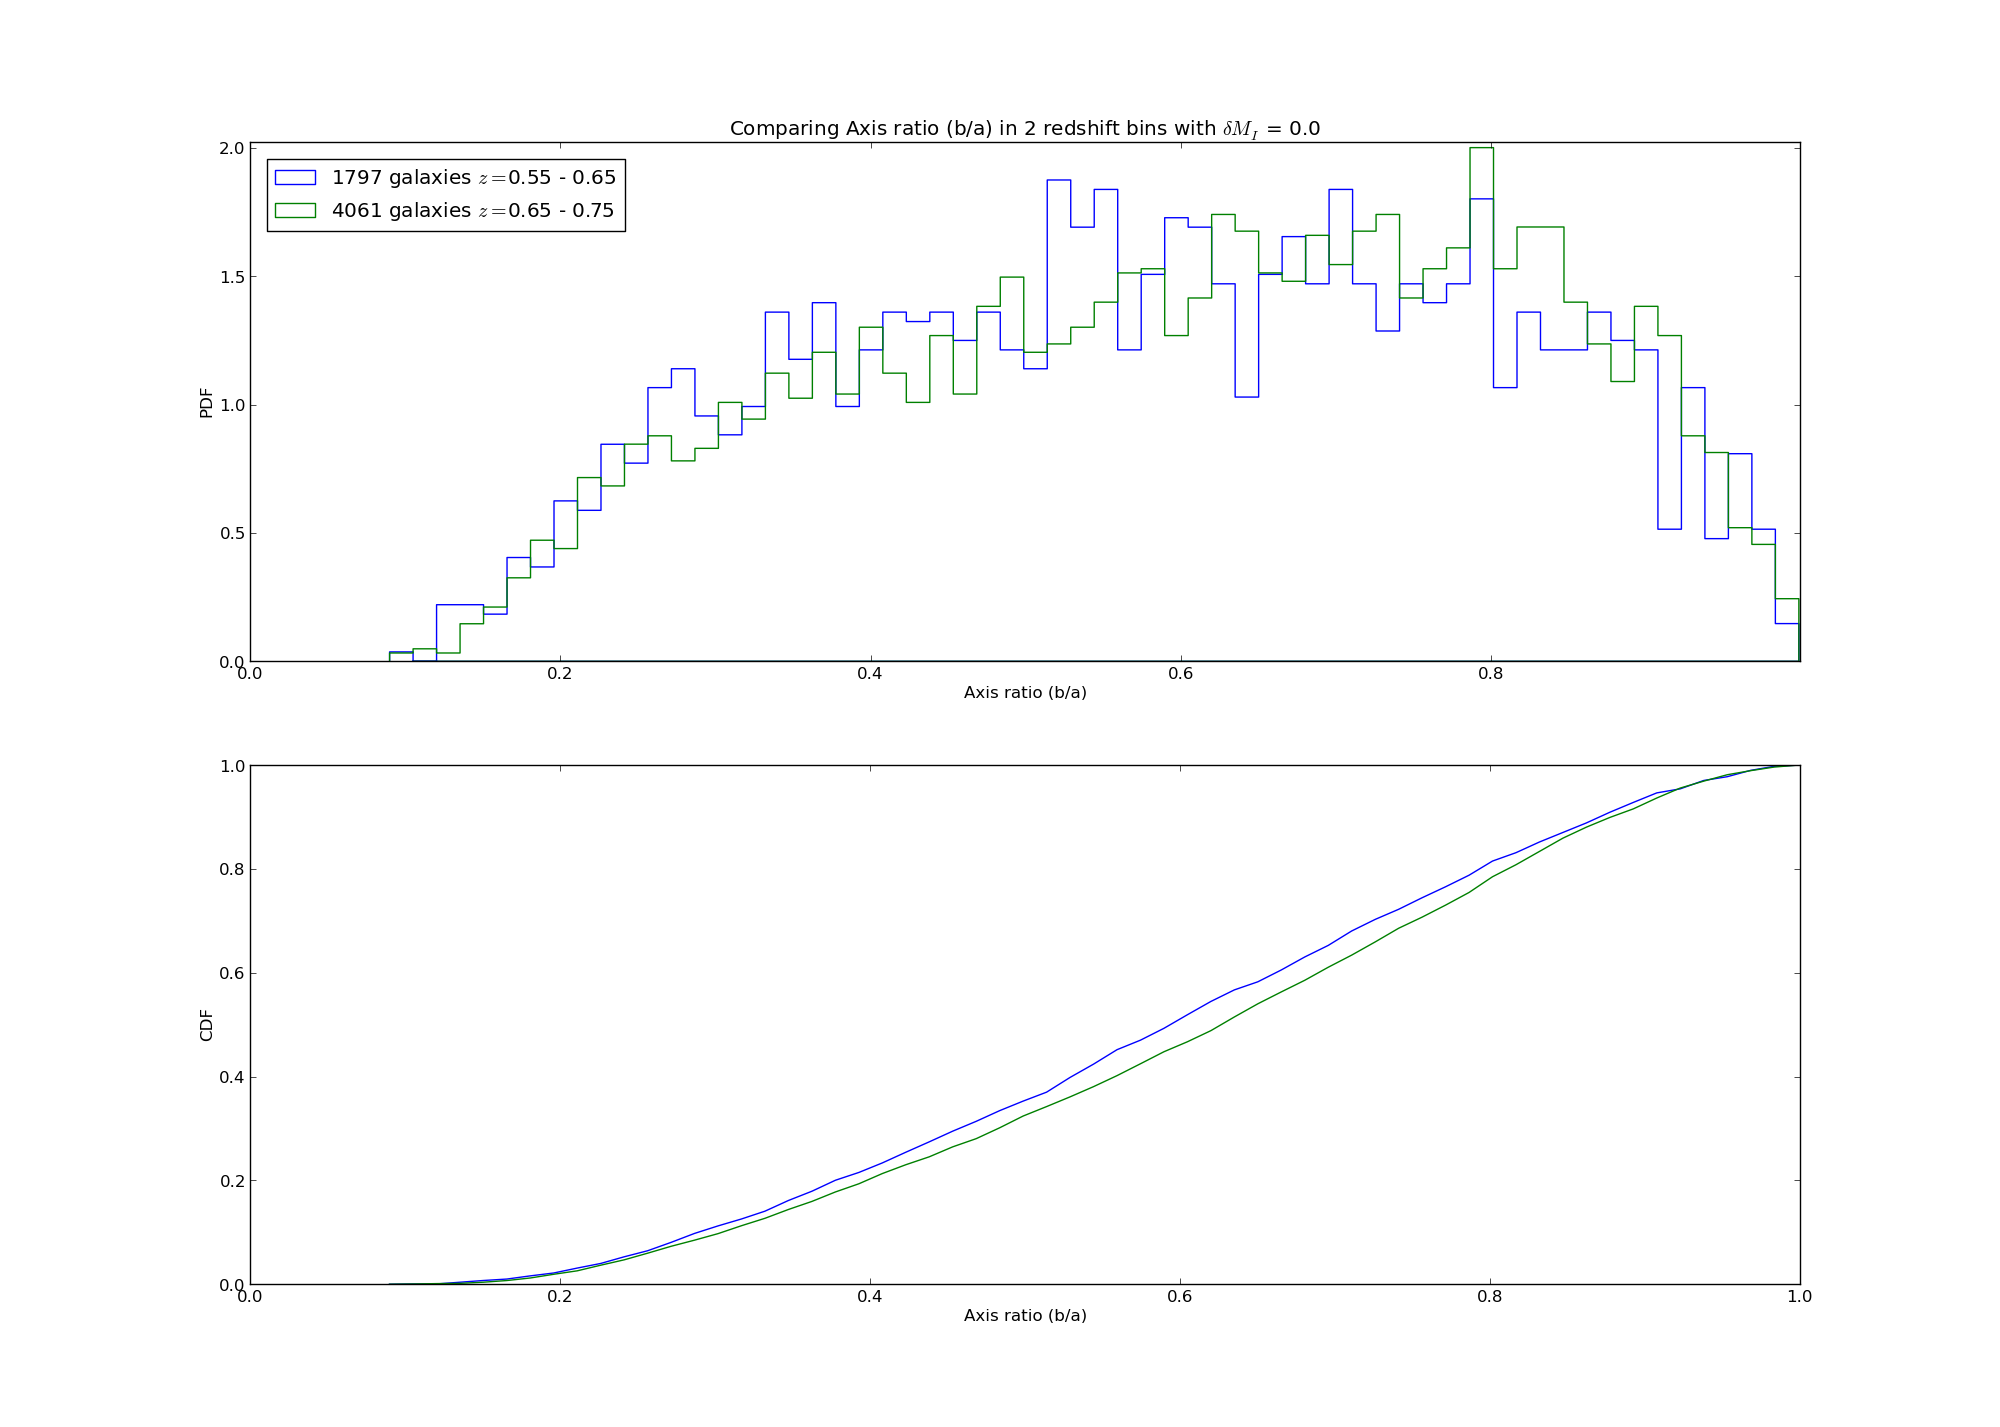
\includegraphics[width=0.9\columnwidth]{axisratio(0)_0dot55-0dot65_0dot65-0dot75.png} \
 b) 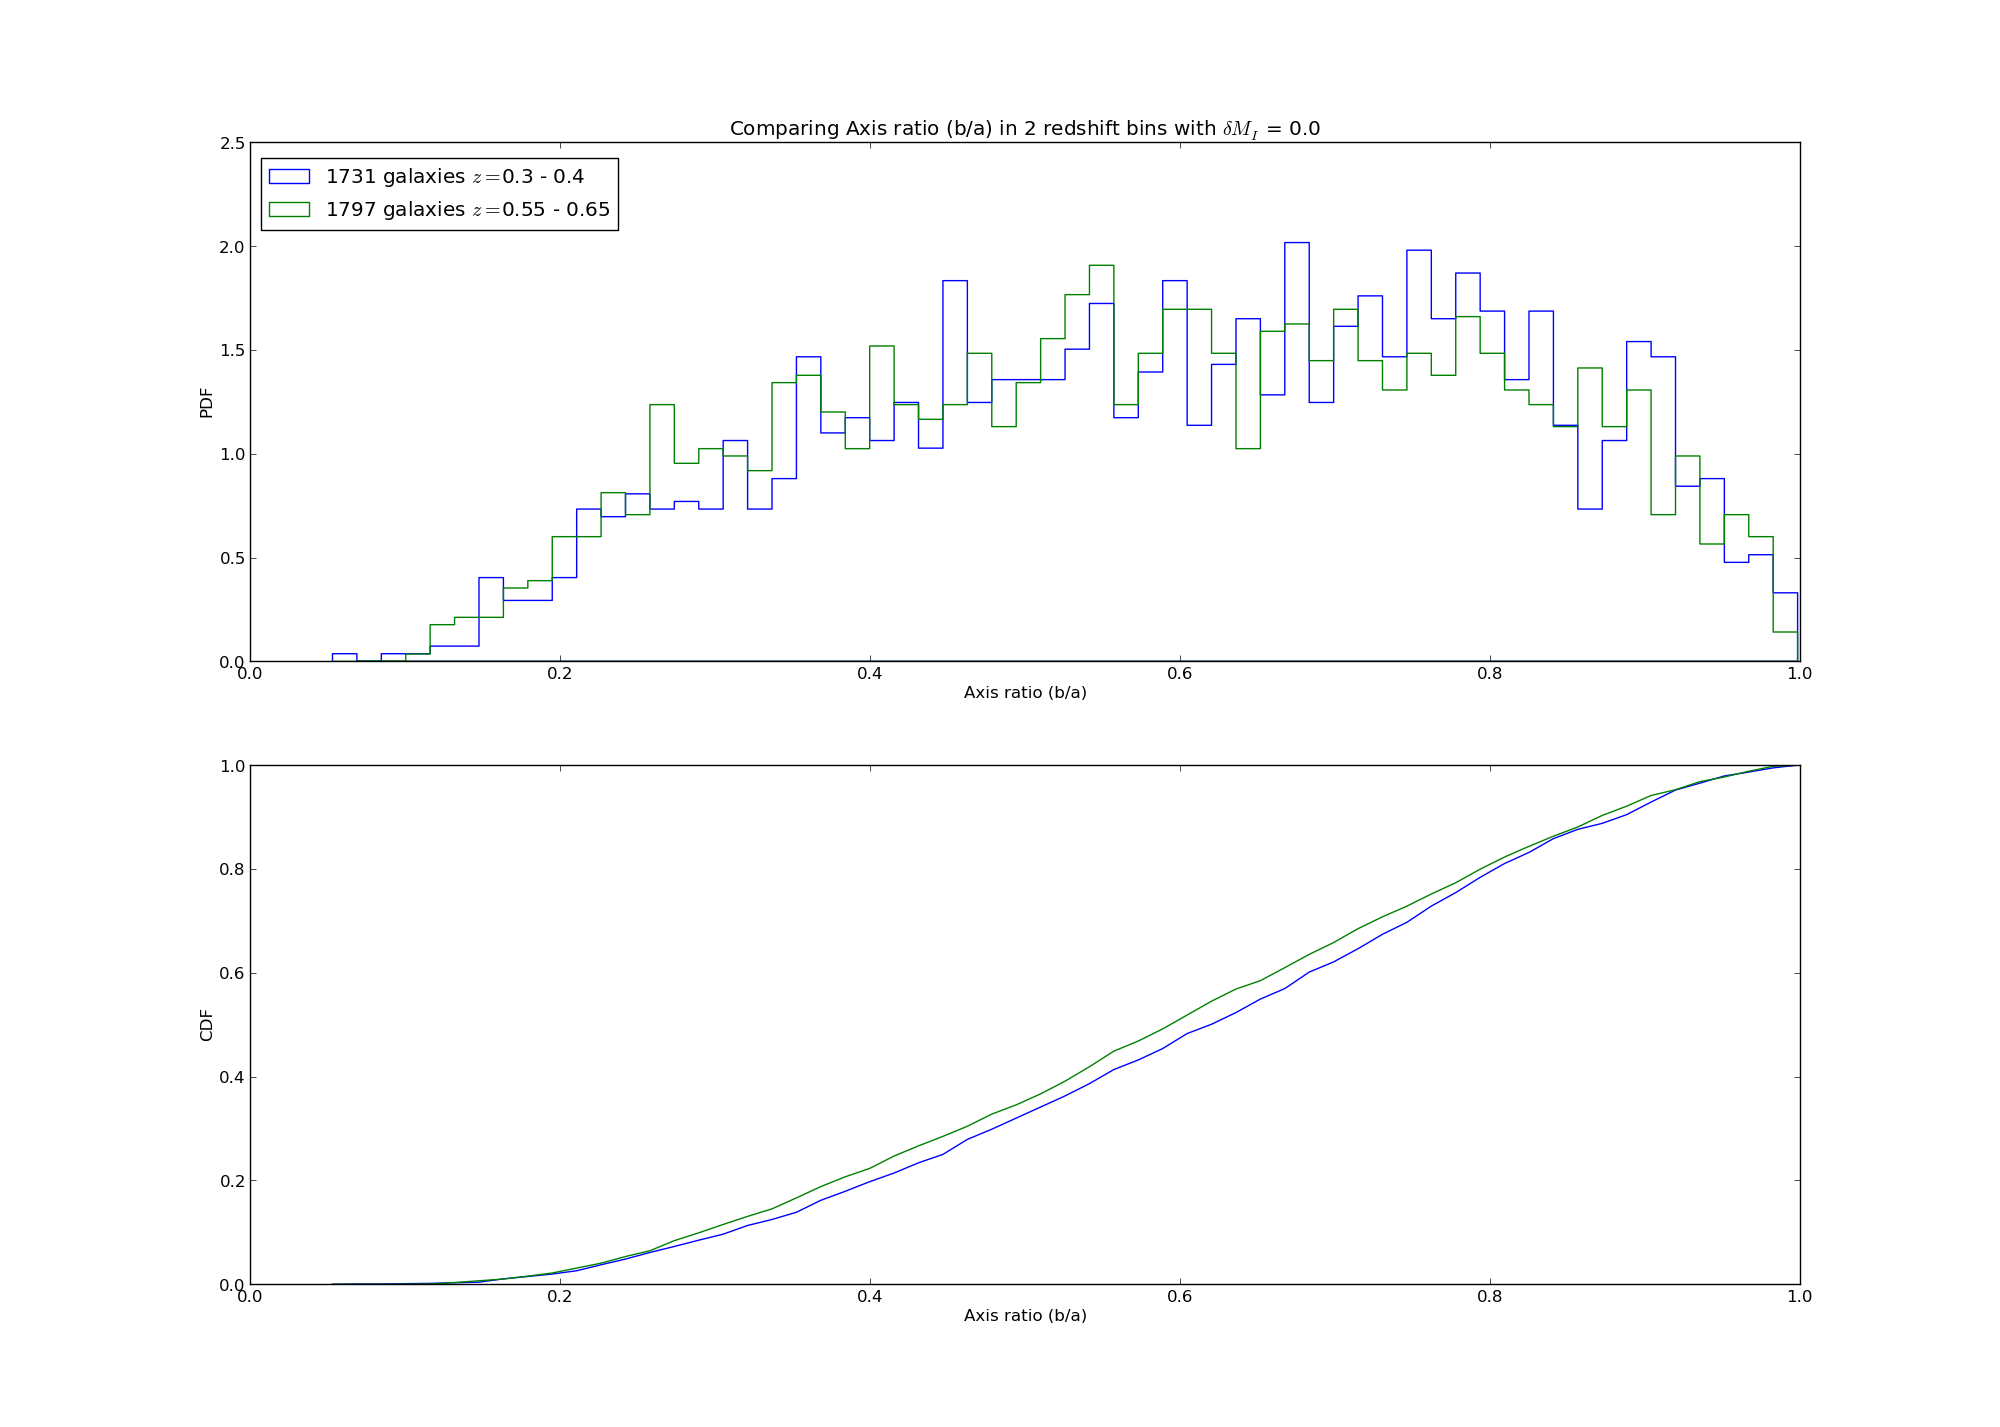
\includegraphics[width=0.9\columnwidth]{axisratio(0)_0dot3-0dot4_0dot55-0dot65.png} \\
 c) 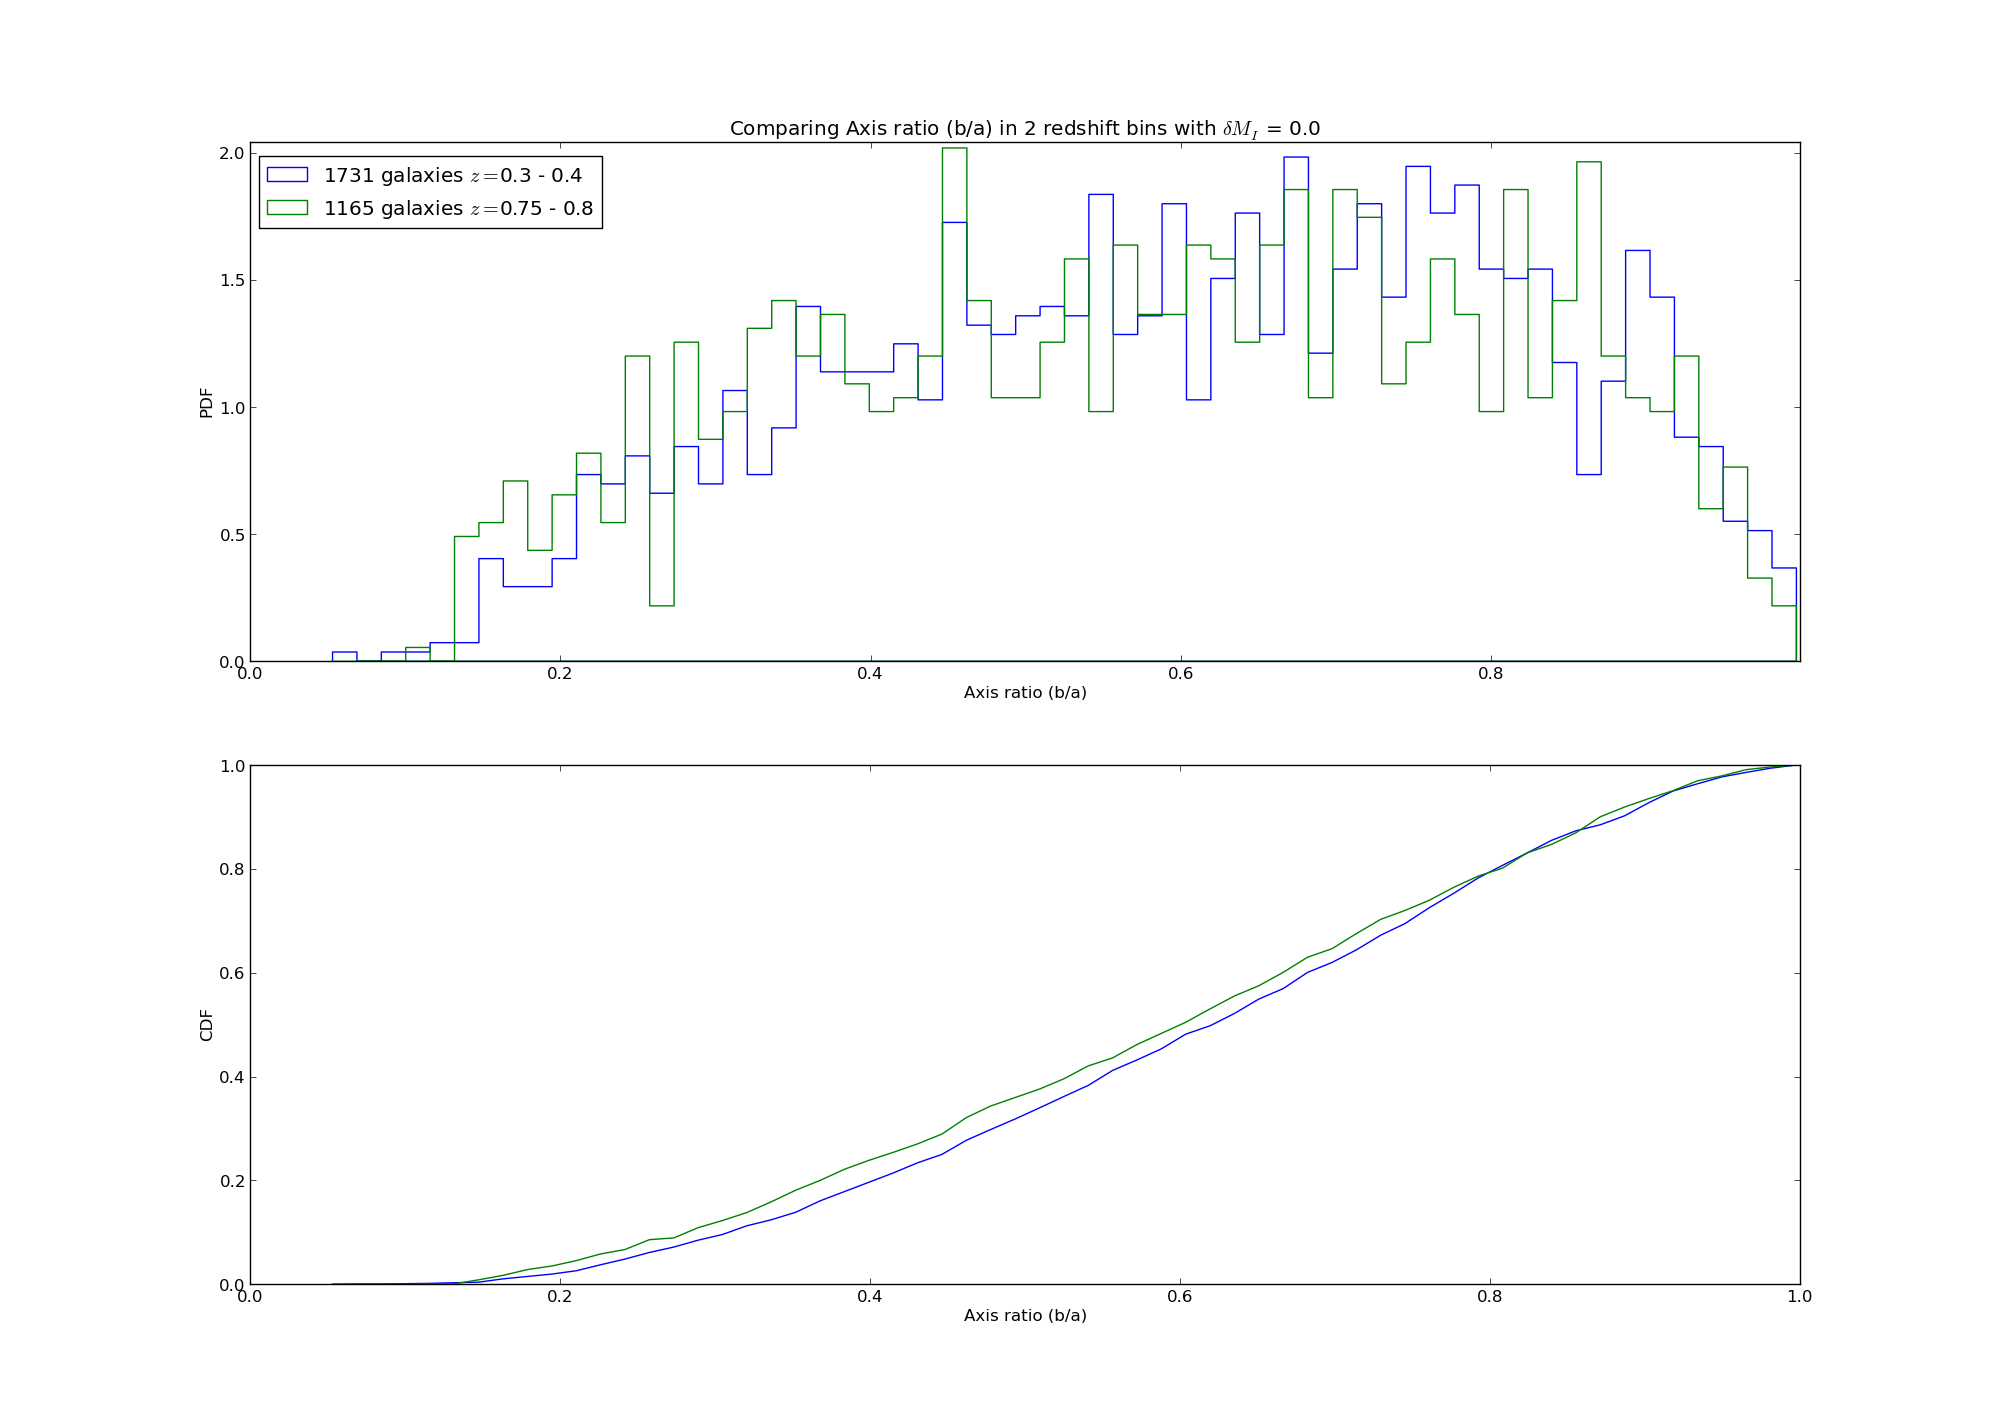
\includegraphics[width=0.9\columnwidth]{axisratio(0)_0dot3-0dot4_0dot75-0dot8.png} \
 d) 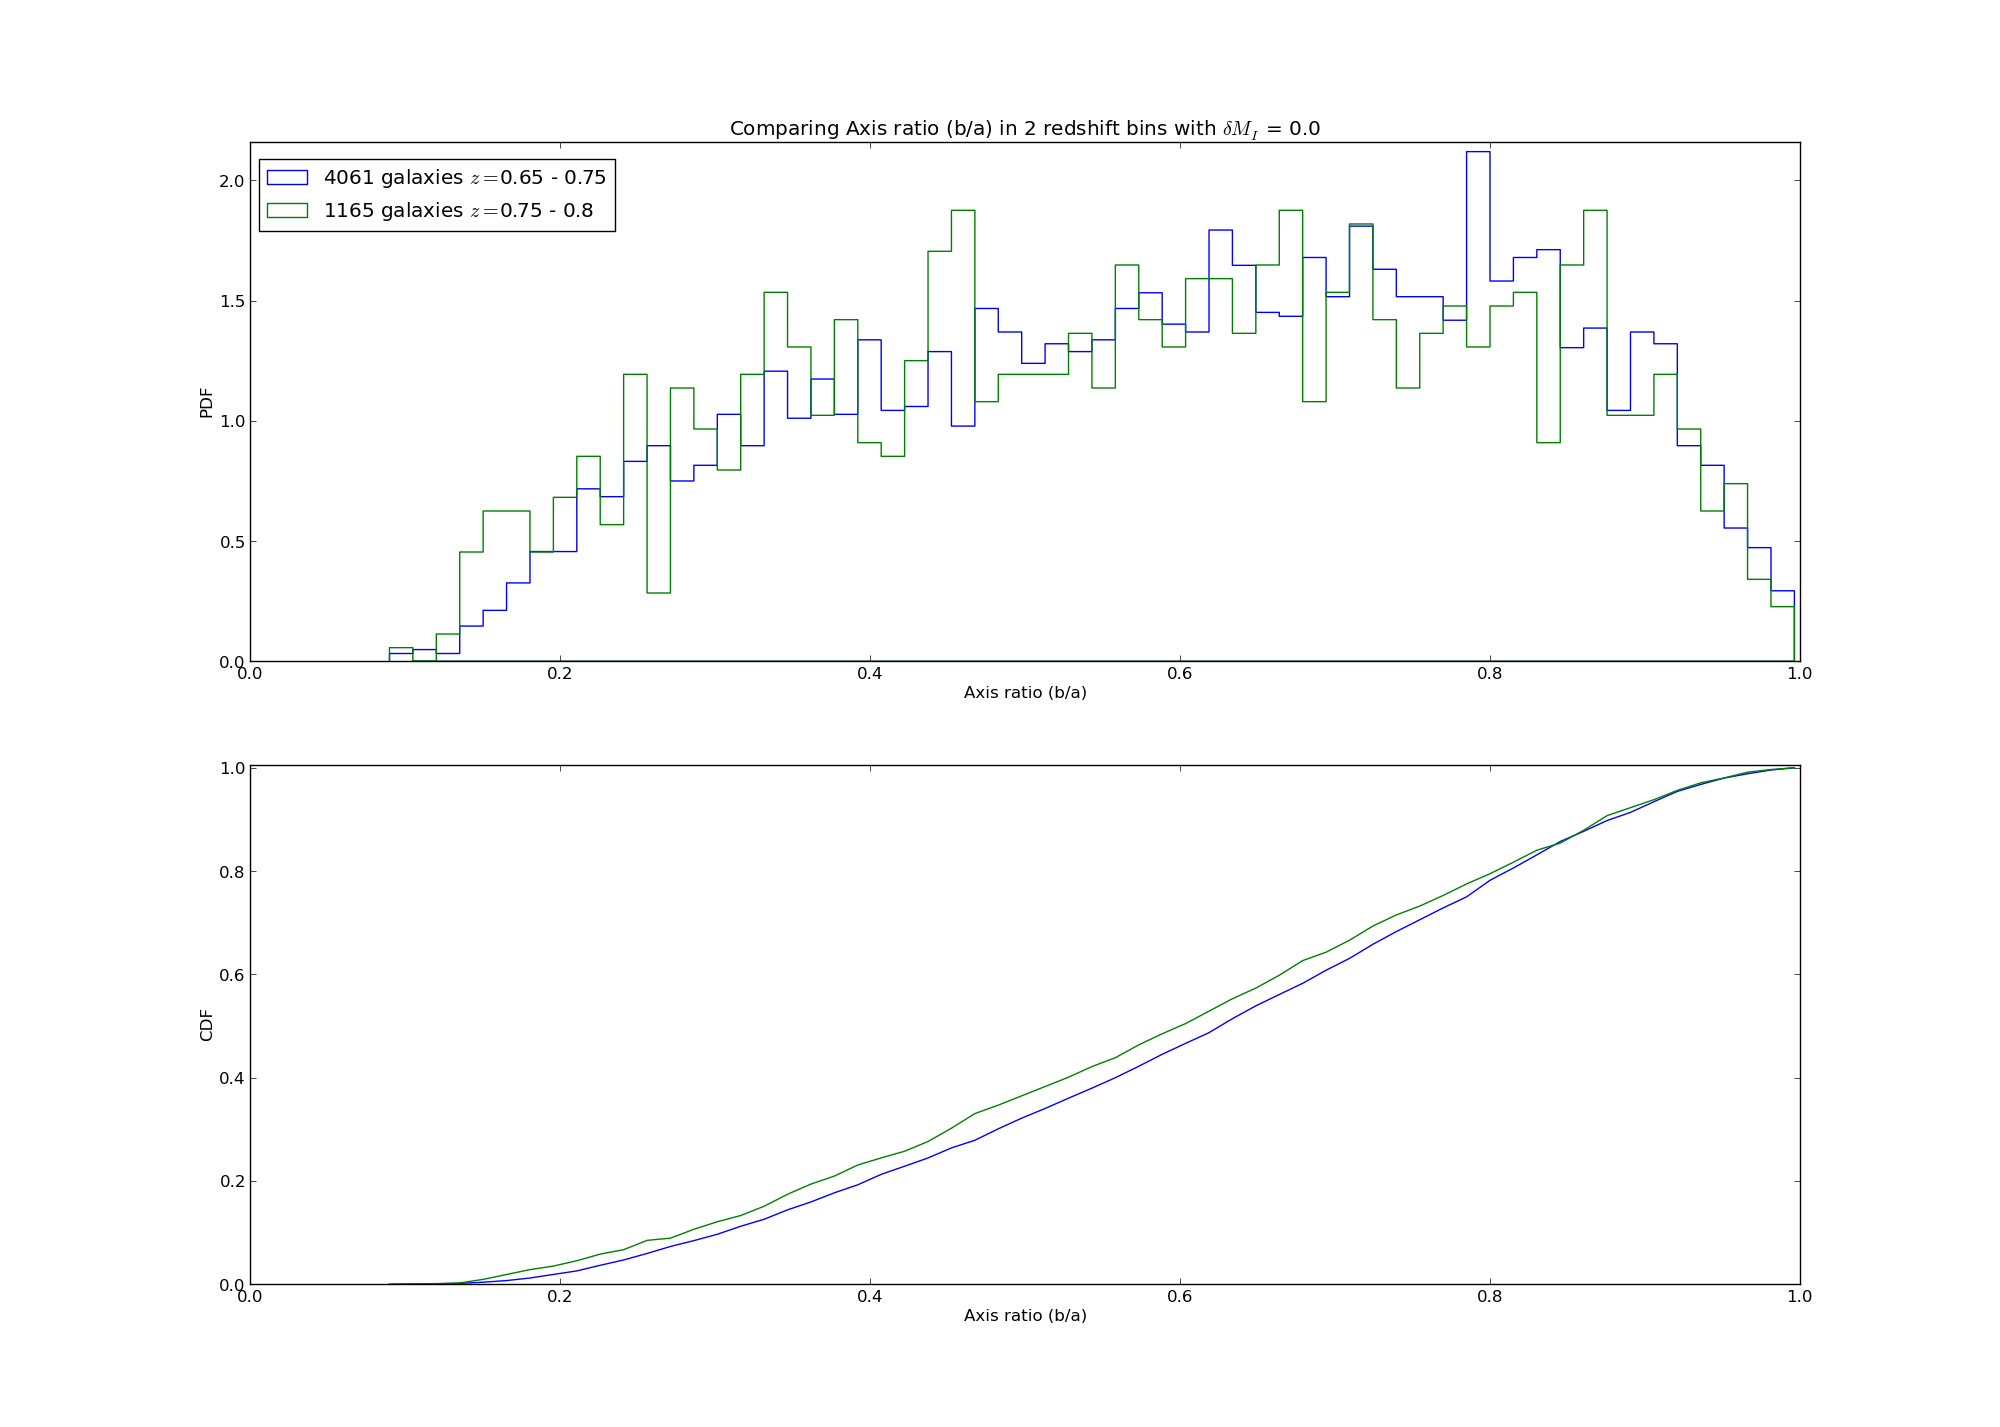
\includegraphics[width=0.9\columnwidth]{axisratio(0)_0dot65-0dot75_0dot75-0dot8.png} \
 \caption{Comparison of axis ratios of galaxies in contrasting environments. $p$-values from the KS and AD test are (will be) given in the plot.}
 \label{fig:axisratio_contrasting}
\end{figure*}

%Figures~\ref{fig:axisratio_similar} and~\ref{fig:axisratio_contrasting} show that the distributions are similar when the environments are similar and different when the environments are different.

%The shape of a population of galaxies can be characterized by a single number called `RMS ellipticity'. If $q=b/a$ is the axis-ratio, then the ellipticity maybe defined as $\frac{1-q}{1+q}$
%or as $\frac{1-q^2}{1+q^2}$. The root mean squared (RMS) of ellipticities of galaxies in each redshift bin are shown in Figure~\ref{fig:rms_ellip}.
It is useful to consider the root mean square ellipticity since it can characterize the shape of the population/sample of galaxies.

\subsection{Comparison plots}

{\bf Insert Fig 6 - All histograms}
In this section, we compare how the intrinsic properties of galaxies vary depending on their environment. In particular, the properties of interest are RMS ellipticity and axis ratios that
characterize the shape of the galaxies, \sersicn and \btt ratio that characterize the morphology of the galaxy, color $M_G - M_I$ since it correlates with galaxy morphology
and Half-light radius that characterizes the size of the galaxies. Our approach would be to compare the distributions of these quantities in two or more redshift bins 
using Kolmogorov-Smirnov and Anderson-Darling test.

Quantitative results of this comparison is presented in {\bf Table 1}. Test statistic and $p$-values are obtained from Kolmogorov-Smirnov test (KS-test)
and 2-sample Anderson-Darling tests (AD-test) are given below

%\begin{enumerate}
% \item KS2 - Kolmogorov-Smirnov 2 sample test on unweighted samples.
% \item ADK2 - Anderson Darlington K sample test on unweighted samples.
% \item KS - Kolmogorov-Smirnov test between the underdense sample and linearly-interpolated empirical CDF of the overdense sample weighted appropriately.
% \item KS2\_recon - Kolmogorov-Smirnov 2 sample test between the underdense sample and a sample drawn from the above mentioned CDF.
% \item ADK2\_recon - Anderson Darlington K sample test between the underdense sample and a sample drawn from the above mentioned CDF.  
%\end{enumerate}

{\bf Table 1 (needs update) } - $p$-value matrix 
\begin{tabular}{||c|c|c||}
 \hline
  Field & KS p-value & AD p-value \\
 \hline 
  Apparent magnitude (m) & 1.972e-86 & 0.0 \\
  $i$-band Luminosity (\mi) & 1.459e-2 & 4.98e-3 \\
  Axis ratio $(b/a)$ & 4.277e-4 & 1e-4\\
  \sersicn & 1.593e-5 & 2e-5\\
  Color $(M_G-M_I)$ & 2.889e-2 & 7.8e-4\\
  
\end{tabular}

Having a conventional threshold for $p$-value $p_{\text{threshold}} = 0.05$, we conclude that the distributions are inconsistent from the above table.
When two randomly partitions of the sample is compared, the distributions are consistent with each other most of the time. The reason why the distributions
do not agree might partly because of the environment and partly because of the evolution with redshift. The subsequent sections are dedicated to separate out
their contributions.

%Average values of quantities of interest are plotted in {\bf Table 2}

%{\bf Table 2 } - Average values.

% \section{Redshift evolution}
% 
% Although randomly partitioned overdense galaxies were in agreement with each other,
% overdense regions at low redshifts are found to be incompatible with the overdense regions at higher redshifts.
% This suggests there could be 

In the subsequent sections, we will compare distributions between two overdense / underdense regions, where we expect to find similarity, and between an overdense and underdense regions,
where we expect the distributions to differ.

The RMS ellipticities of galaxies in each redshift bin are shown in Figure~\ref{fig:rms_ellip}.

\begin{figure*}
 \centering
 a) 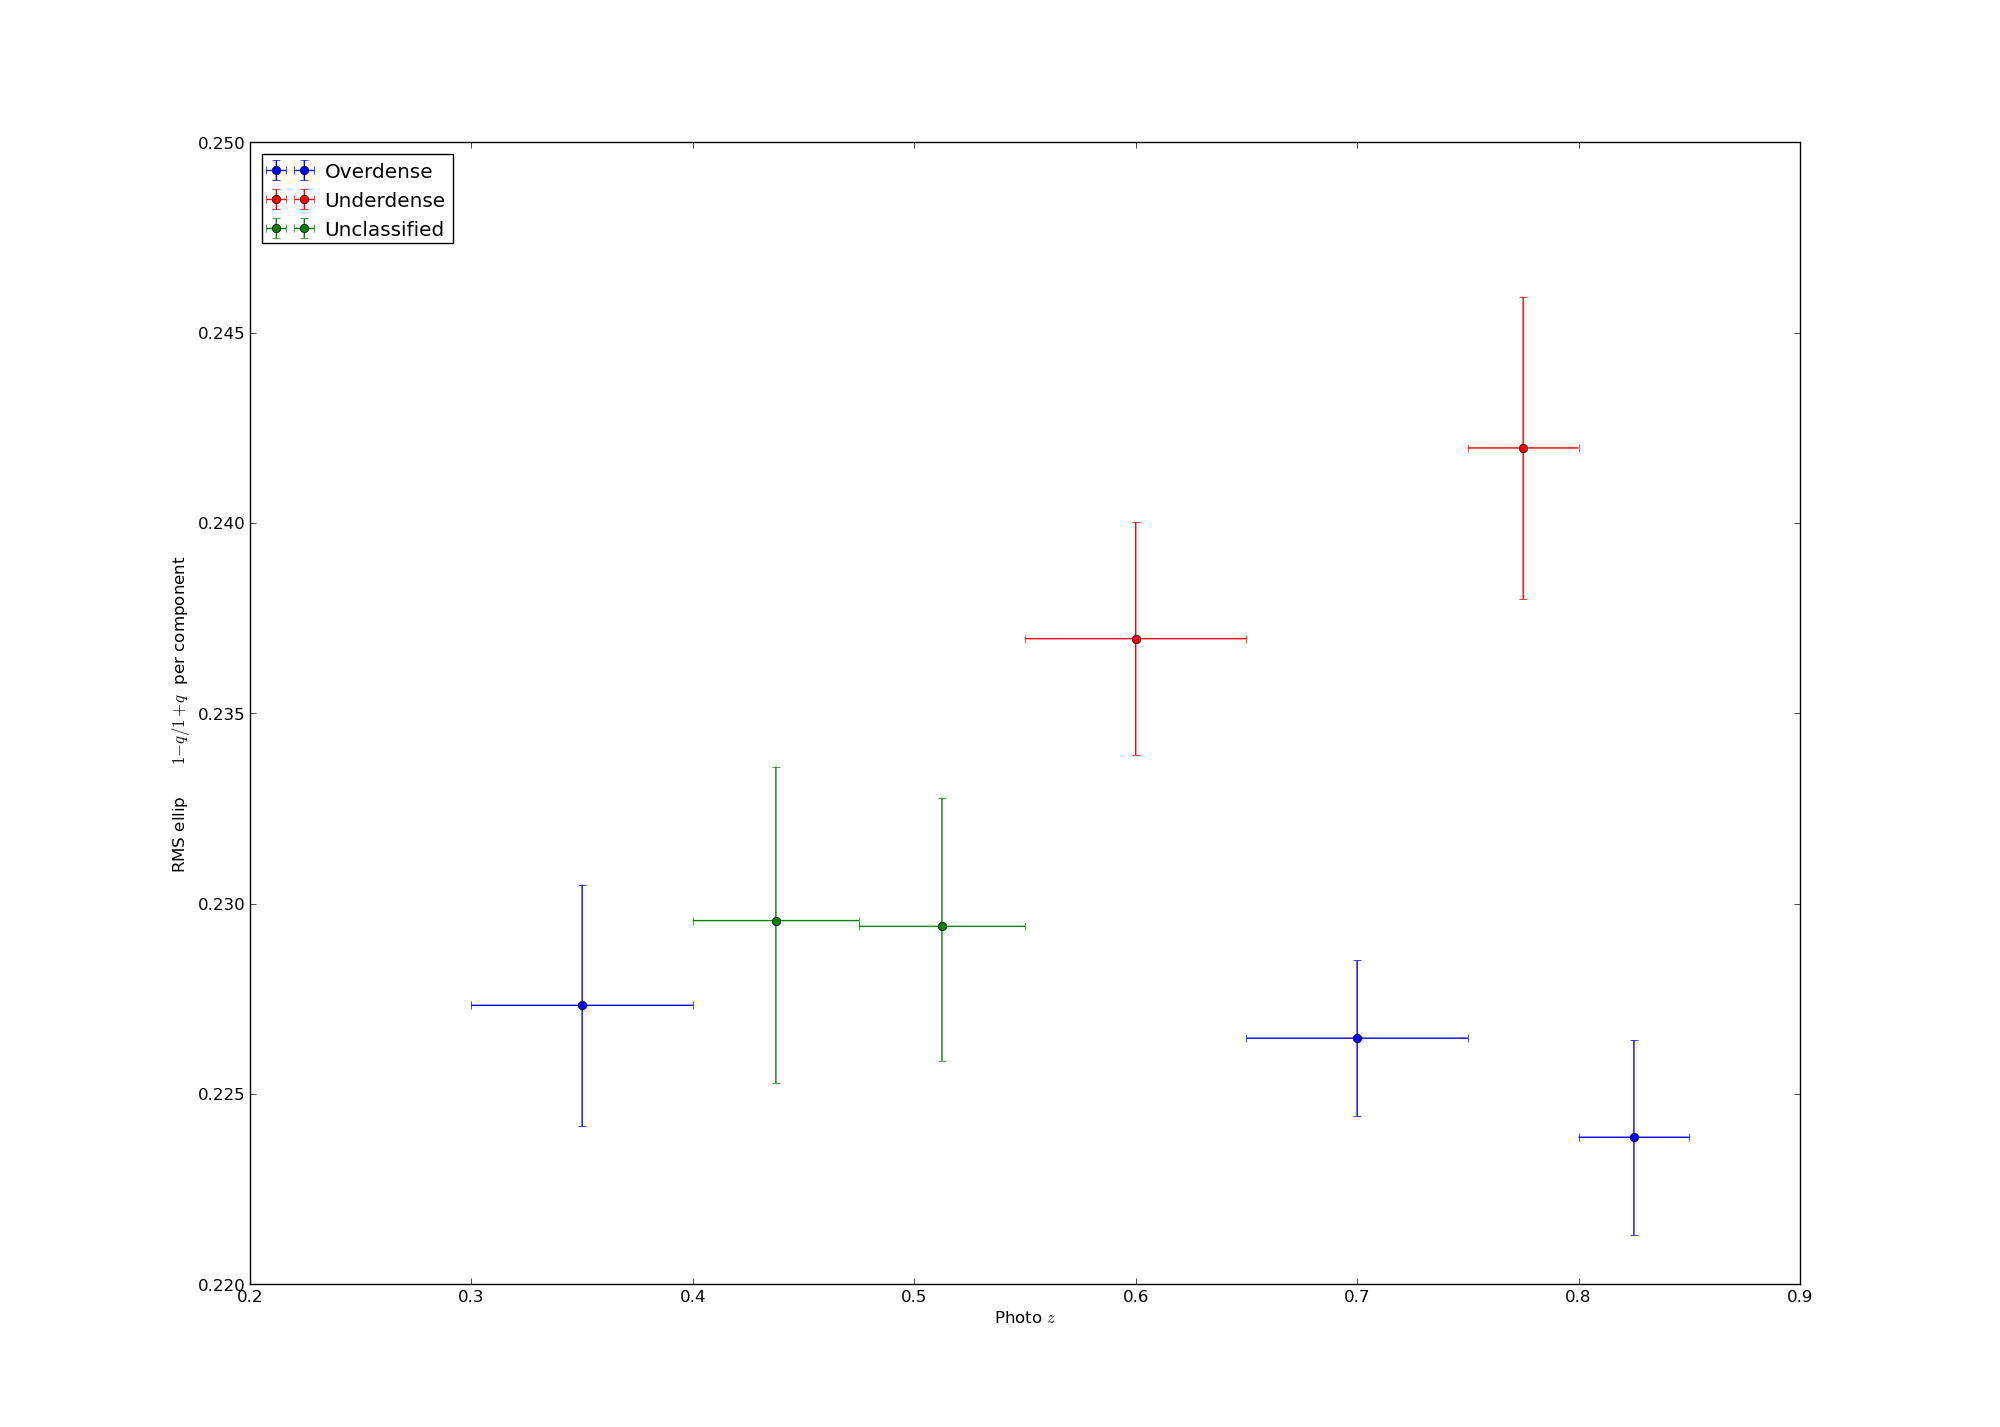
\includegraphics[width=0.9\columnwidth]{rms_ellip1.png} \
 b) 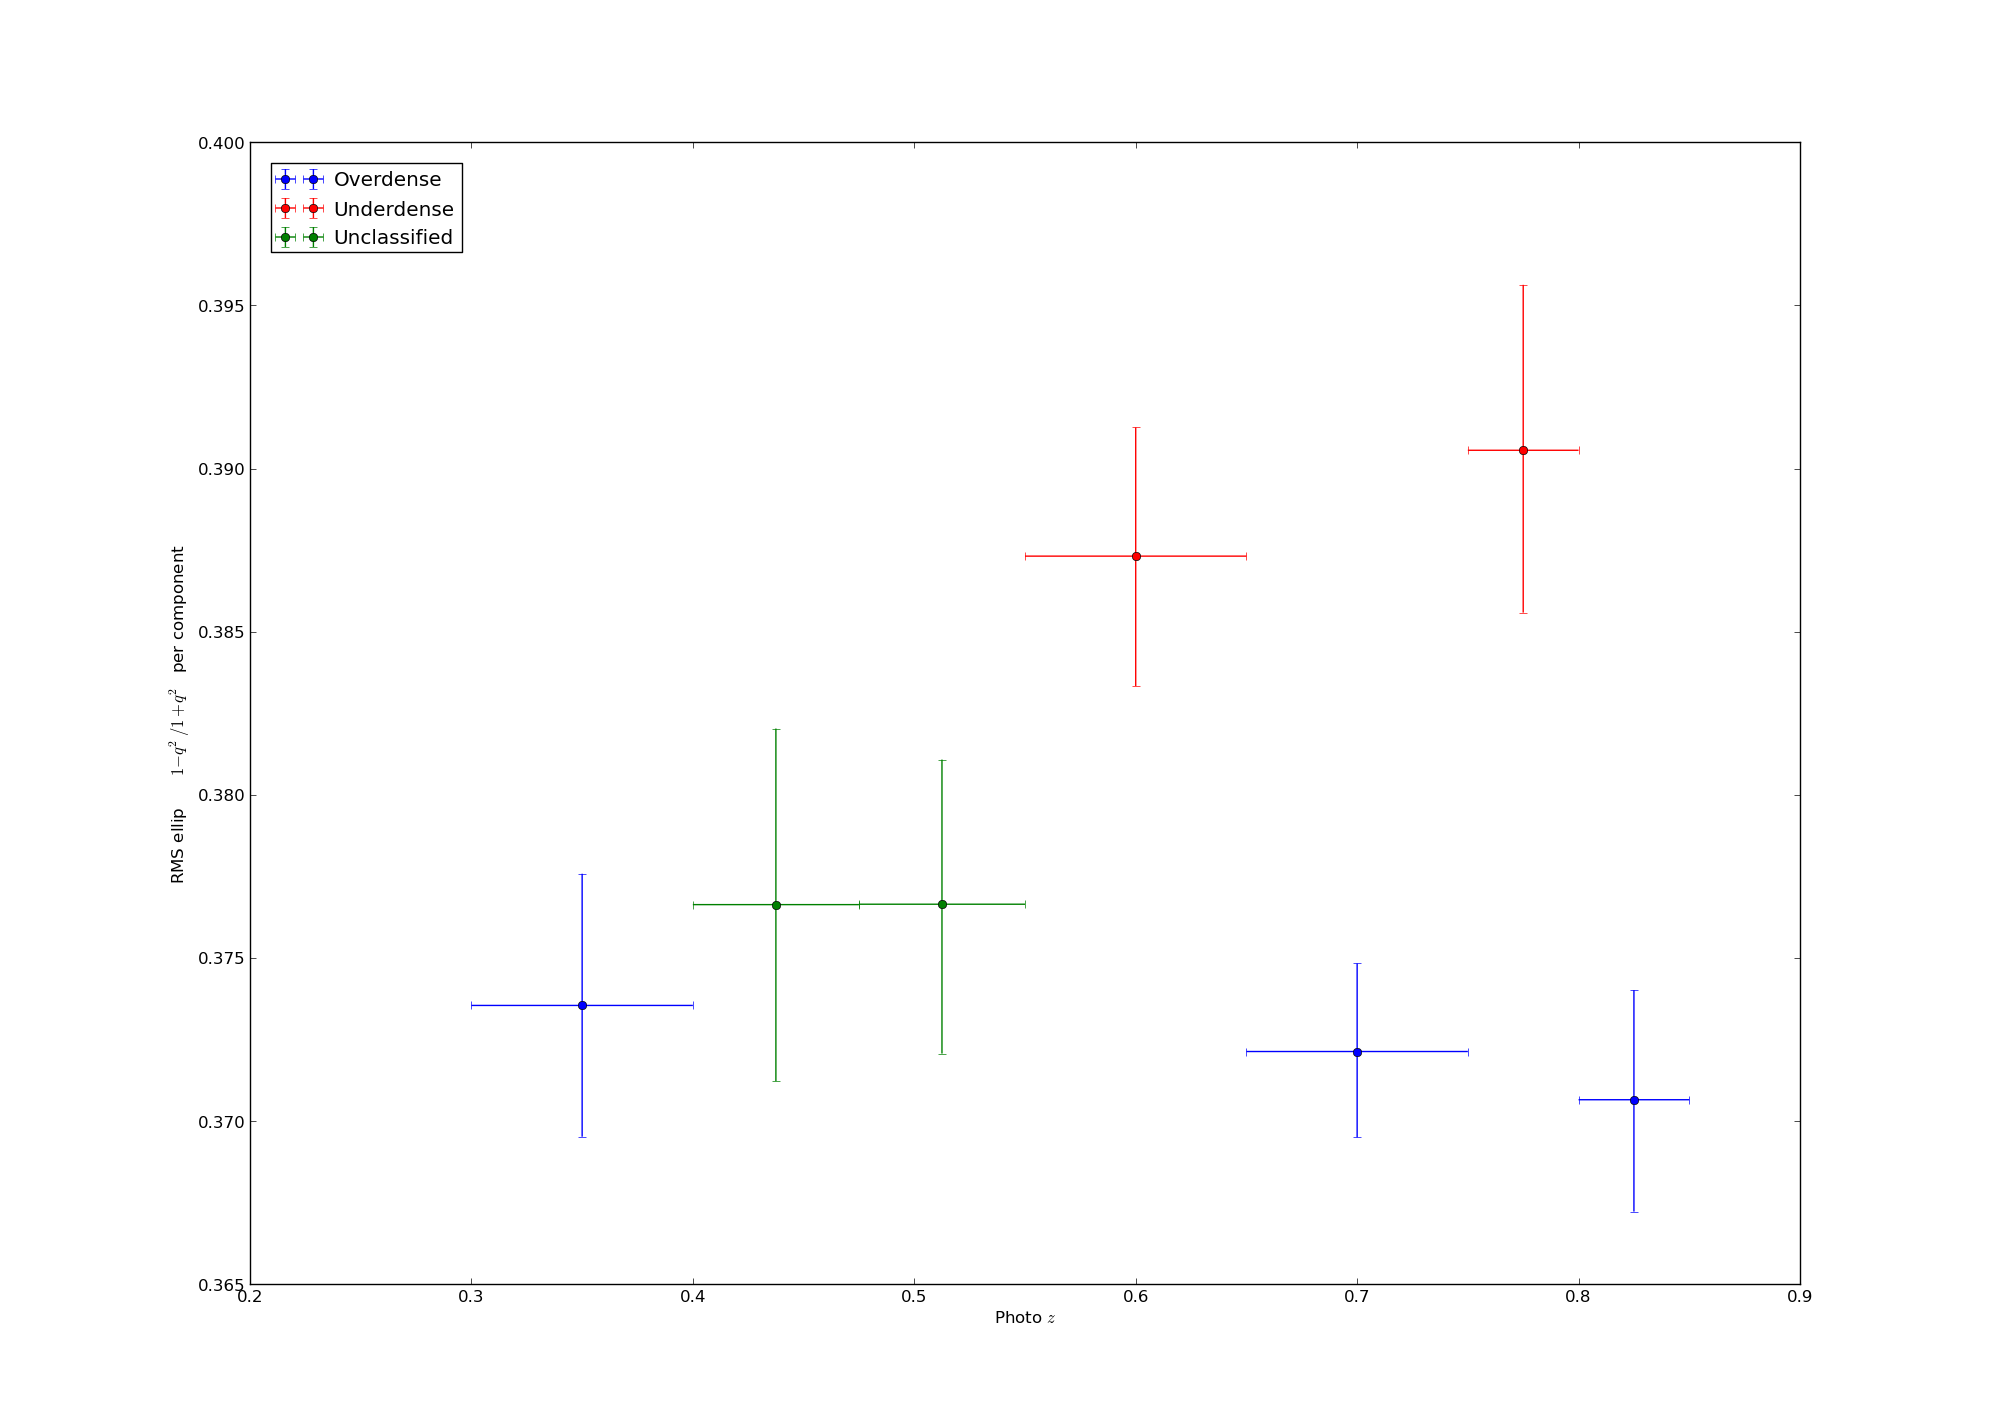
\includegraphics[width=0.9\columnwidth]{rms_ellip2.png} \\
 \label{fig:rms_ellip}
\end{figure*}

\section{Conclusion}

We have shown that 
\section*{Acknowledgments}

AK and RM acknowledge the support of NASA ROSES 12-EUCLID12-0004, and
program HST-AR-12857.01-A, provided by NASA through a grant from the
Space Telescope Science Institute, which is operated by the
Association of Universities for Research in Astronomy, Incorporated,
under NASA contract NAS5-26555

%\begin{thebibliography}
\bibliography{ref}
%\end{thebibliography}

\end{document}


